% !TeX spellcheck = en_GB
% %%% ***************** CHAPTER RESULTS ***************** %%%
\chapter{Results and Discussion} \label{ch:Res}
% \textcolor{red}{\textbf{The overleaf file from the Results is here:} \\ \url{https://www.overleaf.com/15070250fhqztvnygzmn}} 
% \\V
%
In this chapter the results of the surface observation, the optimal estimation retrieval and the regional mesoscale forecast model are presented. On the basis of the methodology described in \Cref{ch:Methods} it should be evaluated if a regional mesoscale forecast model predicts the same synoptic patterns as observed at the measurement site. Also, vertical SWC forecasted by MEPS is being verified with the retrieved vertical SWC at Haukeliseter. Attention should be paid to the fact, that this study study is very unique of its kind. As far as the author has knowledge was no approach done to verify a vertical regional forecast model with the help of vertical observation measurements. 

%%%%%%%%%%%%%%%%%%%%%%%%%%%%%%%%%%%%%%%%%%%%%%%%%%%%%%%%%%%%%%%%%%%%%%%%%%
%%%%%%%%% Observation agreement %%%%%%%%%%%%%%
\section{Comparison of surface observations} 
%%%%%%% image scatter obs ret %%%%%%%%%%%%%%%%
\begin{figure}[t]
	\centering
	\begin{subfigure}[b]{0.38\textwidth}
		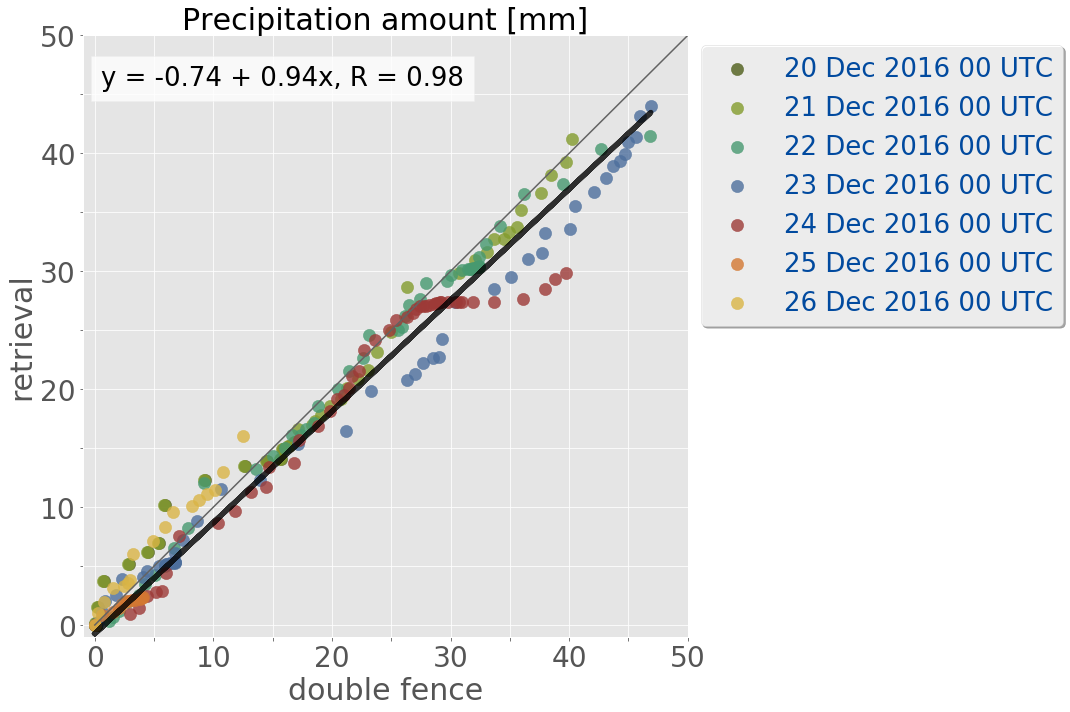
\includegraphics[trim={0.cm 0.cm 13cm 0cm},clip,
		width=\textwidth]{./fig_obs_ret/obs_ret_20161220_26_00}
		\caption{}\label{fig:res:obs_ret_scatter}
	\end{subfigure}
	%
	\begin{subfigure}[b]{0.59\textwidth}
		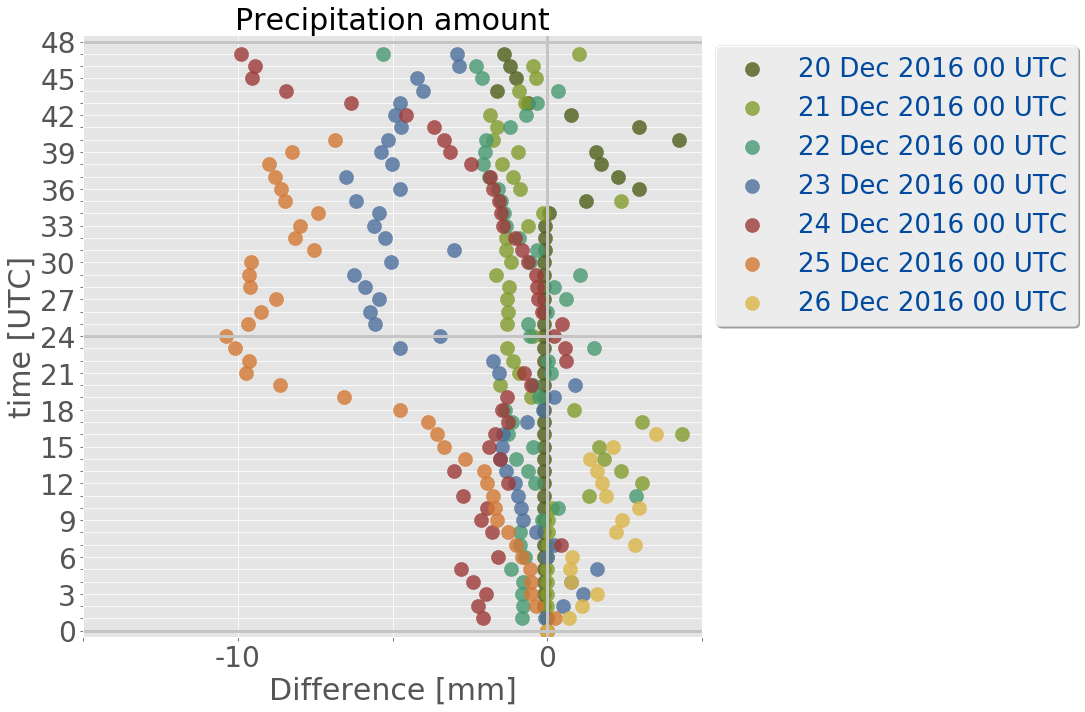
\includegraphics[trim={0.cm 0.cm 0cm 0cm},clip,
		width=\textwidth]{./fig_obs_ret/diff_20161220_26_00}
		\caption{}\label{fig:res:diff_ret_scatter}
	\end{subfigure}
	% label
	%    \begin{subfigure}[t]{0.18\textwidth}
	%   	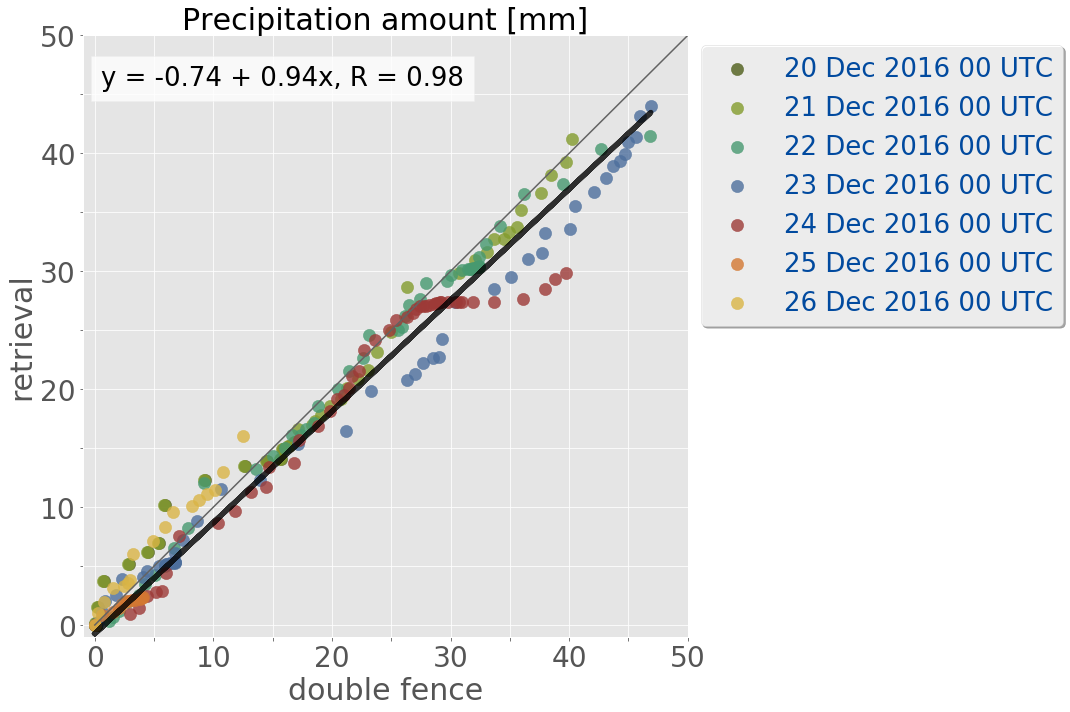
\includegraphics[trim={25.cm 13.cm 0cm 1.3cm},clip,
	%  width=\textwidth]{./fig_obs_ret/obs_ret_20161220_26_00}
	% \end{subfigure}
	\caption{\protect\subref{fig:res:obs_ret_scatter}: Surface precipitation amount comparison between the double fence observations and the retrieved surface accumulation of precipitation for \SI{48}{\hour}. In black the linear correlation between the double fence observations and retrieved surface snow. 
    \protect\subref{fig:res:diff_ret_scatter}: Difference between the retrieved and the observed accumulation by the double fence. The colours represent the different starting days at \SI{0}{\UTC} for the \SI{48}{\hour} accumulation.}\label{fig:res:obs_ret}
\end{figure}
%%%%%%%%%%%%%%%%%%%%%%%%%%%%%%%%%%%%%%%%%%%%%%
To be able to compare the vertical predicted snow water content with the retrieved snow water content a verification of the surface accumulation is made. If the retrieved surface accumulation is confident in comparison to the double fence measurement, then the vertical measurements can be trusted.
\\
The correlation in \Cref{fig:res:obs_ret_scatter} demonstrates a good agreement between the \SI{48}{\hour} accumulation measured by the double fence and the retrieved surface accumulation.
The black line in \Cref{fig:res:obs_ret_scatter} presents a linear correlation with a regression coefficient of R = \num{0.97}. 
In general, the retrieved surface snowfall accumulation is underestimated when compared to the double fence measurements, but not to a large degree. 
\\
\Cref{fig:res:diff_ret_scatter} shows the difference between retrieved accumulation and observed accumulation by the double fence. For the time period \num{20} to \SI{24}{\dec}, \Cref{fig:res:diff_ret_scatter} indicates an underestimation of retrieved snow accumulation of less than \SI{-5}{\mm} for the first \SI{24}{\hour}. 
Snow accumulation calculated on \SI{23}{\dec} at \SI{0}{\UTC} show after \SI{24}{\hour} an underestimation by the retrieval of up to \SI{-6.5}{\mm}. Larger underestimation after \SI{43}{\hour} is related to the observation of liquid precipitation on \SI{25}{\dec} between \SIrange{12}{21}{\UTC} for accumulations on \SI{24}{\dec}. On \SI{25}{\dec} no fair comparison to the double fence measurement can be performed after \SI{12}{\UTC} because of the neglection of liquid precipitation when temperatures exceed \SI{2}{\celsius}.
\\
%The mean absolute difference of all days is \SI{2.06}{\mm} (excluding values on \SI{25}{\dec} after \SI{12}{\UTC} and on \SI{26}{\dec} after \SI{17}{\UTC} because of attenuation at the MRR). 
For a \SI{12}{\hour} accumulation follows for the Christmas storm (\num{20} to \SI{26}{\dec}) an average error of \SI{85.5}{\percent} (\Cref{tab:res:ret_error}). For longer, \SI{24}{\hour} accumulation decreases the average error to be \SI{- 4.7}{\percent} (excluding values on \SI{25}{\dec} after \SI{12}{\UTC} and on \SI{26}{\dec} after \SI{17}{\UTC} because of attenuation at the MRR). The daily surface snowfall accumulation difference between retrieval and observation in \Cref{tab:res:ret_error} show almost always a well agreement to the boundary condition of the double fence. The only well pronounced mismatch is seen non \SI{21}{\dec}, where it measures much more than the double fence gauge (+\SI{435.8}{\percent}). 
\\
Similar to this study, \citet{cooper_variational_2017} used a CloudSat snow particle model, PSD and fall speed from MASC observations for five snow events at Barrow, Alaska. The comparison to the weather station revealed an difference between National Weather Service observations and retrieved accumulations of \SI{- 18}{\percent} for all five snow events.
%%%%%%% table error sfc acc ret obs %%%%%%%%%%%%%%%%
\begin{table}[t!]
	\begin{center}
		\caption{Comparison of observed (obs.) and retrieved (ret.) snowfall amounts for the Christmas storm 2016. Difference refers to the difference of the retrieved and observed snow accumulation after \SI{12}{\hour} and \SI{24}{\hour}. The average difference is the value over all six/four days. Excluding values after \SI{12}{\UTC} on \SI{25}{\dec} and after \SI{17}{\UTC} on \SI{26}{\dec}.}\label{tab:res:ret_error}
		\begin{tabular}{c||r|r|c|c||c|c|c|c}
			\hline \hline
			& \multicolumn{4}{c||}{\textbf{\SI{12}{\hour} accumulation}} & \multicolumn{4}{c}{\textbf{\SI{24}{\hour} accumulation}}    \\ \cline{2-9}
            \textbf{Day} & \multicolumn{2}{c|}{\textbf{Snowfall}} & \textbf{Difference} & \textbf{Average} &  \multicolumn{2}{c|}{\textbf{Snowfall}} & \textbf{Difference} & \textbf{Average}  \\\cline{2-3} \cline{6-7}
            \textbf{in 2016} & \textbf{obs.} & \textbf{ret.} & & \textbf{difference} & \textbf{obs.} & \textbf{ret.} & & \textbf{difference} \\\cline{2-9}
			& \multicolumn{2}{c|}{[\SI{}{\mm}]} & [\SI{}{\percent}] & [\SI{}{\percent}] & \multicolumn{2}{c|}{[\SI{}{\mm}]} & [\SI{}{\percent}] & [\SI{}{\percent}] \\ \hline\hline
			\num{20} Dec & \num{0.1} &\num{0.0} & \num{-97.8} & & \num{0.1} & \num{0.0} & \num{- 97.8} &  \\\cline{1-9}
			\num{21} Dec & \num{0.7} & \num{3.8} & +\num{435.8} & \multirow{6}{*}{+\num{85.5}} & \num{17.1} & \num{16.6} & \num{-2.7} & \multirow{4}{*}{\num{-4.7}}   \\\cline{1-4}\cline{6-8}
			\num{22} Dec & \num{13.6}& \num{13.2} & \num{- 3.0} & & \num{25.6} &\num{25.1} & \num{-2.1} &   \\\cline{1-4}\cline{6-8}
			\num{23} Dec & \num{6.3} &\num{5.2} & \num{- 16.8} & & \num{23.3}& \num{19.8} & \num{-14.9} &   \\\cline{1-4}\cline{6-8}
			\num{24} Dec & \num{14.7} & \num{13.4} & \num{- 8.6} && \num{24.8} & \num{25.0} & +\num{0.8} &   \\\cline{1-4}\cline{6-9}
			\num{25} Dec &  \num{4.3} & -- & -- & & +\num{15.4} & -- & -- & \\\cline{1-4}\cline{6-9}
			\num{26} Dec & \num{8.8} & \num{10.6} & +\num{20.1} &  &  \num{25.1} &-- & -- &  \\\hline\hline
		\end{tabular}
	\end{center}
\end{table}
%%%%%%%%%%%%%%%%%%%%%%%%%%%%%%%%%%%%%%%%%%%%%%
\\
\Cref{tab:res:ret_error} shows the difference for each individual day and the average difference for six and 4 days, depending on the accumulation of \SI{12}{\hour} or \SI{24}{\hour}.
The choice of the correct PSD model, slope parameters and fall speed in the optimal estimation snowfall retrieval, shows a good agreement with the observations at Haukeliseter for the 2016 Christmas storm in contrast to the \SI{200}{\percent} difference when only using the CloudSat snowfall algorithm \Cref{sec:retrieval}. It indicates also that the non-uniqueness of snow accumulation is reduced, when using a combination of ground-based observations instead of only Ze-S relationships. 
%Of course, more storms should be investigated to find the exact correlation between the surface observations and the estimated accumulation to see if the deviation keeps as small for different snow patterns at Haukeliseter. 
During the 2016 Christmas storm the average error for \SI{24}{\hour} accumulation is almost similar to Barrow, Alaska. It turns out that there is no relation between high and low precipitation events since the differences vary. \citet{cooper_variational_2017} also showed different combinations of PSD assumptions and snow fall speed. For Barrow, best agreements between observations and retrieved snowfall were found by using the CloudSat particle model, slope parameters and snowfall speeds from the MASC. The here presented work (\Cref{sec:retrieval}) uses a particle model based on observed particle sizes during the entire winter 2016/2017, like in \Cref{fig:MASC}. \textcolor{red}{Add Discussion on different combination/parameters as discussed with Steve. }
\\
\\
On \num{20} and \SI{21}{\dec}, the difference error is large (\SI{-97.8}{\percent} and \SI{435.8}{\percent}, respectively). This is probably related to an observation of precipitation at the double fence, even though no precipitation was observed. The double fence observation might be related to some particles stirred up by wind into the orifice of the gauge. Since no manual observations are done at the Haukeliseter site, is it difficult to say if blowing snow occurred and might introduce additional errors. But from the vertical MRR reflectivity it can be seen, that precipitation was not observed on before \SI{21}{\dec} \SI{9}{\UTC}.
\\
Even though it is assumed that the double fence is the absolute correct measurement it still underlies some uncertainties. 
A better way to asses the accuracy of the retrieved surface snowfall accumulation could be to compare the results to measurements inside a bush gage. A bush gauge is a precipitation gauge surrounded by a large bush to create artificial calm winds to increase the catch ratio of frozen precipitation and is considered as the best available measurement for solid precipitation \citep{wolff_wmo_2018}. Unfortunately there are only two bush gauges in the world, and because of local limitations a double fence construction is developed as reference for the Solid Precipitation Measurement intercomparison study during \numrange{1986}{1993} \citep{goodison_wmo_1998}. Comparisons between bush gauge and double fence precipitation measurements have shown, that for wind speeds up to \SI{9}{\mPs} outside the fence, the double fence will measure up to \SI{10}{\percent} less precipitation. 
While wind speeds outside the double fence might reach \SI{20}{\mPs} show measurements inside a decrease to \SI{5}{\mPs}. \citet{wolff_wmo_2018} believes the underestimation of the double fence will not be more than \SI{20}{\percent} during frozen precipitation events with high wind speeds. 
\\
The low average difference value for \SI{24}{\hour} accumulation, in \Cref{tab:res:ret_error} during the Christmas 2016 event (\SI{-4.7}{\percent}) follows a much lower average difference between retrieved and observed surface accumulation than at Barrow (\SI{36}{\percent}) and therefore a very good agreement between observed and retrieved snow accumulation during \num{21} to \SI{24}{\dec}. In \Cref{sec:res:verticalSWC}, the vertical SWC will be compared to the forecasted MEPS values for the 2016 Christmas storm. Despite the condition that the double fence measurement is influenced by wind will the small average difference for \num{21} to \SI{24}{\dec} give confidence in the retrieved profiles of snow water content when comparing to the forecast, but it should be kept in mind that retrieved snow accumulation is underestimated and therefore may the vertical SWC be too low.
%%%%%%%%%%%%%%%%%%%%%%%%%%%%%%%%%%%%%%%%%%%%%%%%%%%%%%%%%%%%%%%%%%%%%%%%%%

%%%%%%%%%%%%%%%%%%%%%%%%%%%%%%%%%%%%%%%%%%%%%%%%%%%%%%%%%%%%%%%%%%%%%%%%%%
%%%%%%%%% Synoptic Phenomena observed? %%%%%%%%%%%%%%
\section{Observation and predictions of large scale weather phenomena at the surface}\label{sec:res:large_scale_sfc}
One of the main factors, that made the Christmas 2016 storm so interesting is the fact, that fronts passed over Norway during the six-day period. One aim of this work is to determine if large scale features were observed at the measurement site during the extreme event. 
\\
A comparison between the surface observations at Haukeliseter and the ECMWF analysis of the dynamic tropopause and geopotential thickness maps show that frontal passages occurred on three days during the Christmas storm (\Cref{fig:GeopJet} and \ref{fig:DynTropo}).  
%These frontal boundaries show in the surface observations and ensemble forecasts on \SIlist{23;25;26}{\dec}. 
A typical cyclone has a prevailing warm front and a faster moving cold front. As the storm gets more intense and the cold front rotates around the low-pressure centre and catches the warm front the cyclone will begin to occlude. Changes in pressures, temperature, wind direction and wind speed can occur. In some cases, an intensification of the precipitation can be observed as well.
\\
\Cref{fig:res:sfc_obs_meps} shows the different parameters forecasts initialised at \SI{00}{\UTC} for \SIlist{23;25;26}{\dec}, as well as the observations at the Haukeliseter measurement site in dash-red.
Typical pressure decreases and increases, as well as temperature increases, and wind changes are present on \SIlist{23;26}{\dec}, since these changes show in the surface observations in \Cref{fig:res:sfc_obs_meps}, it is assumed that frontal boundaries passed. The \SI{25}{\dec} shows only an increase of temperature leading to the assumption of a warm air passage in \Cref{fig:res:sfc_temp25}.
%%%%%%% image sfc obs  %%%%%%%%%%%%%%%%
\begin{figure}[H]
	\centering
	% sfc pressure
	\begin{subfigure}[b]{0.49\textwidth}
		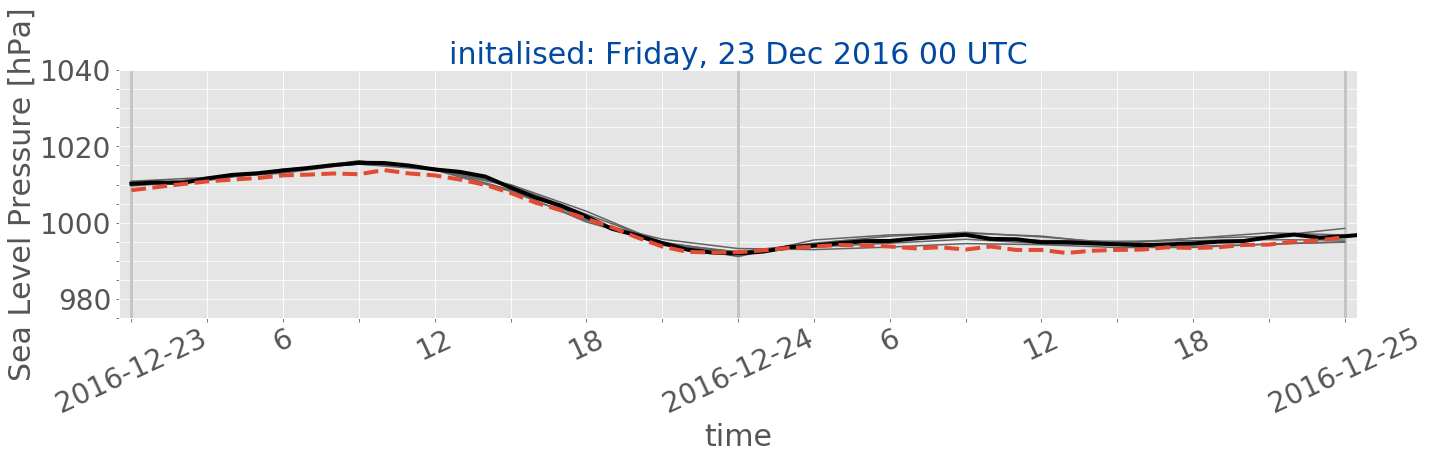
\includegraphics[trim={0.cm 5.cm 0cm 0cm},clip,
		width=\textwidth]{./fig_sfc_pressure/20161223_00}
		\caption{}\label{fig:res:sfc_pres23}
	\end{subfigure}
	%
	\begin{subfigure}[b]{0.49\textwidth}
		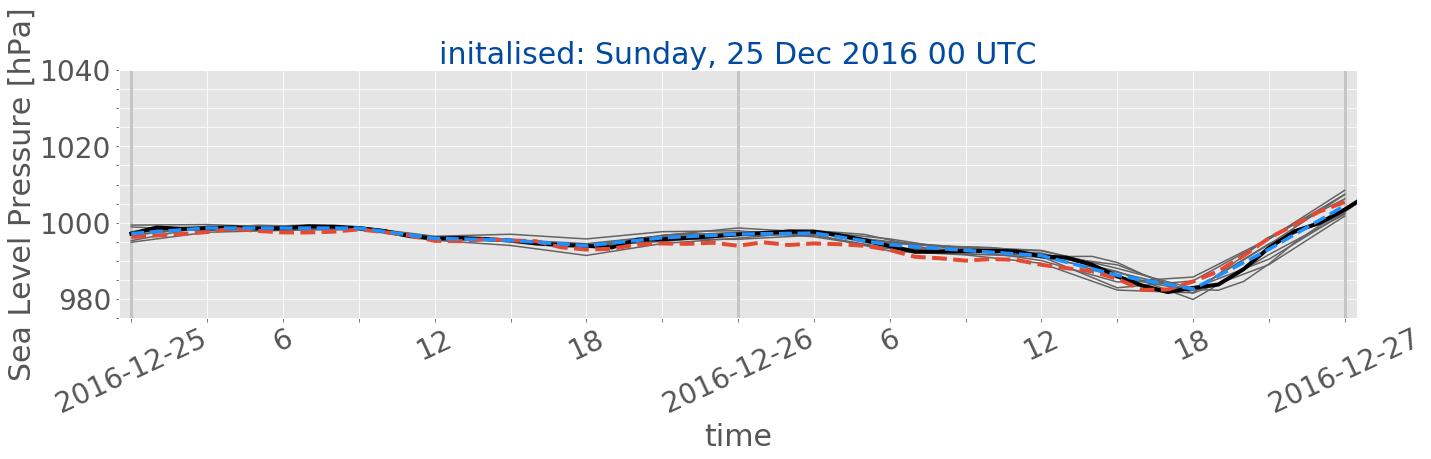
\includegraphics[trim={0.cm 5.cm 0cm 0cm},clip,
		width=\textwidth]{./fig_sfc_pressure/20161225_00}
		\caption{}\label{fig:res:sfc_pres25}
	\end{subfigure}
	% sfc temp
	\begin{subfigure}[b]{0.49\textwidth}
		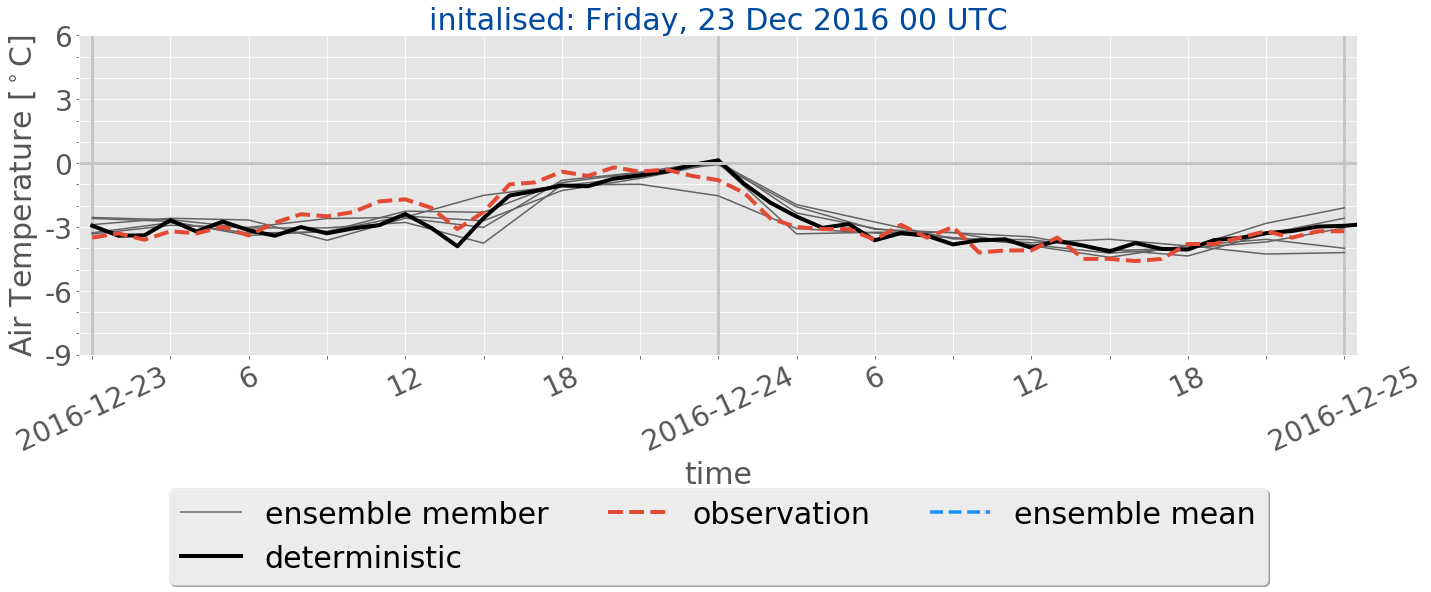
\includegraphics[trim={0.cm 5.cm 0cm 0cm},clip,
		width=\textwidth]{./fig_sfc_temp/20161223_00}
		\caption{}\label{fig:res:sfc_temp23}
	\end{subfigure}
	%
	\begin{subfigure}[b]{0.49\textwidth}
		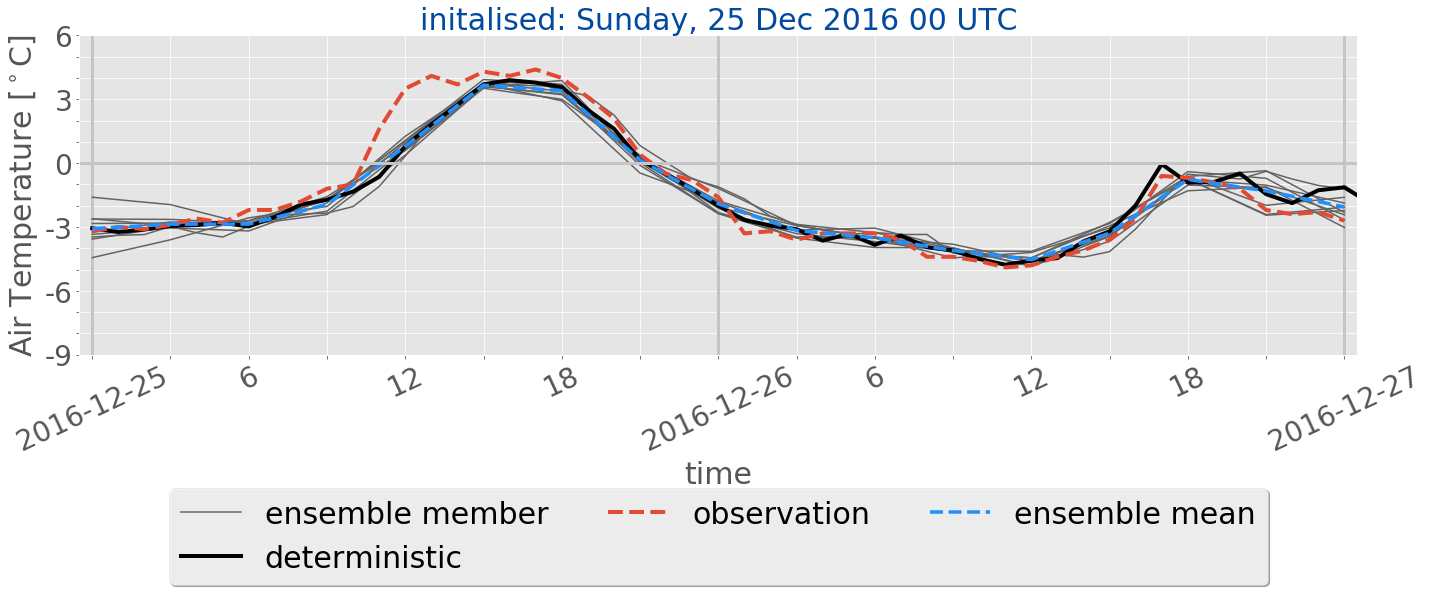
\includegraphics[trim={0.cm 5.cm 0cm 0cm},clip,
		width=\textwidth]{./fig_sfc_temp/20161225_00}
		\caption{}\label{fig:res:sfc_temp25}
	\end{subfigure}
	% sfc wd
	\begin{subfigure}[b]{0.49\textwidth}
		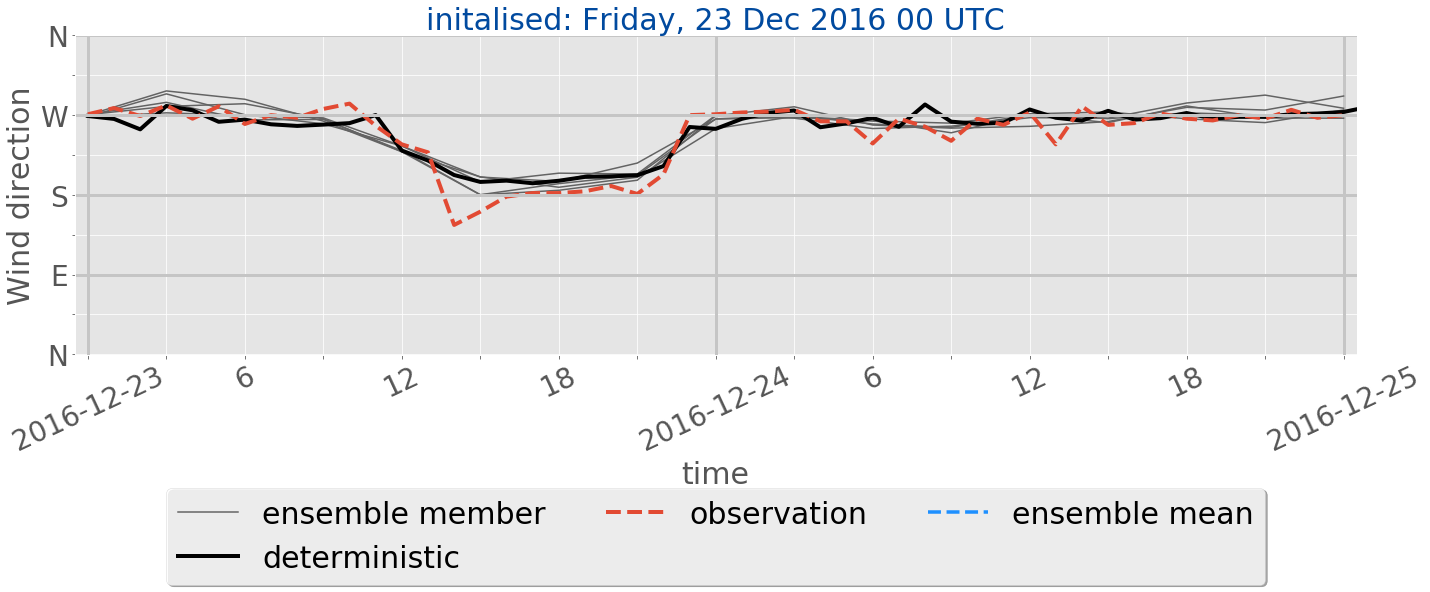
\includegraphics[trim={0.cm 5.cm 0cm 0cm},clip,
		width=\textwidth]{./fig_sfc_wd/20161223_00}
		\caption{}\label{fig:res:sfc_wd23}
	\end{subfigure}
	%
	\begin{subfigure}[b]{0.49\textwidth}
		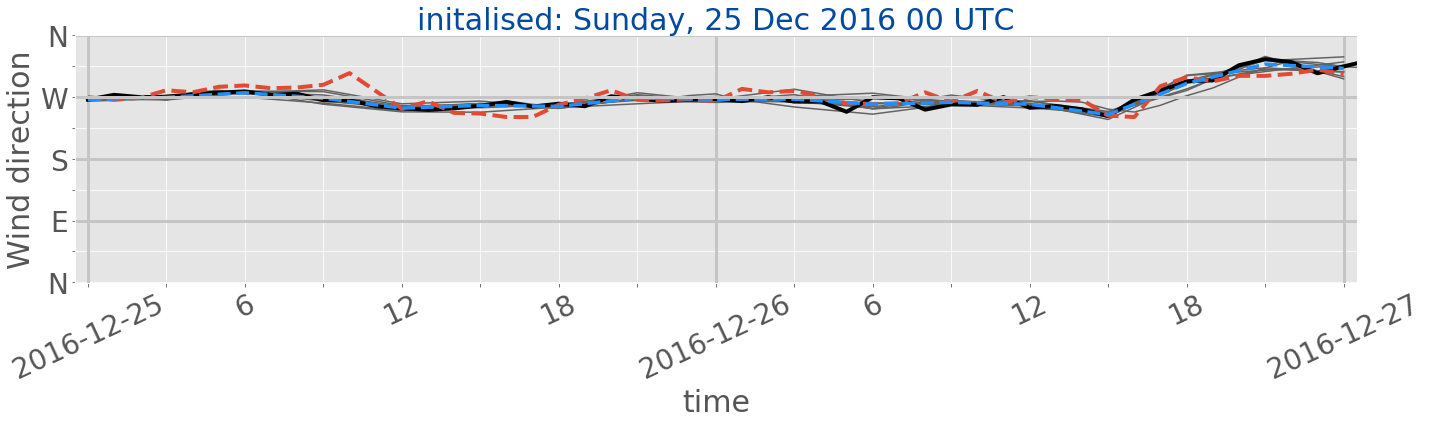
\includegraphics[trim={0.cm 5.cm 0cm 0cm},clip,
		width=\textwidth]{./fig_sfc_wd/20161225_00}
		\caption{}\label{fig:res:sfc_wd25}
	\end{subfigure}
	% sfc ws
	\begin{subfigure}[b]{0.49\textwidth}
		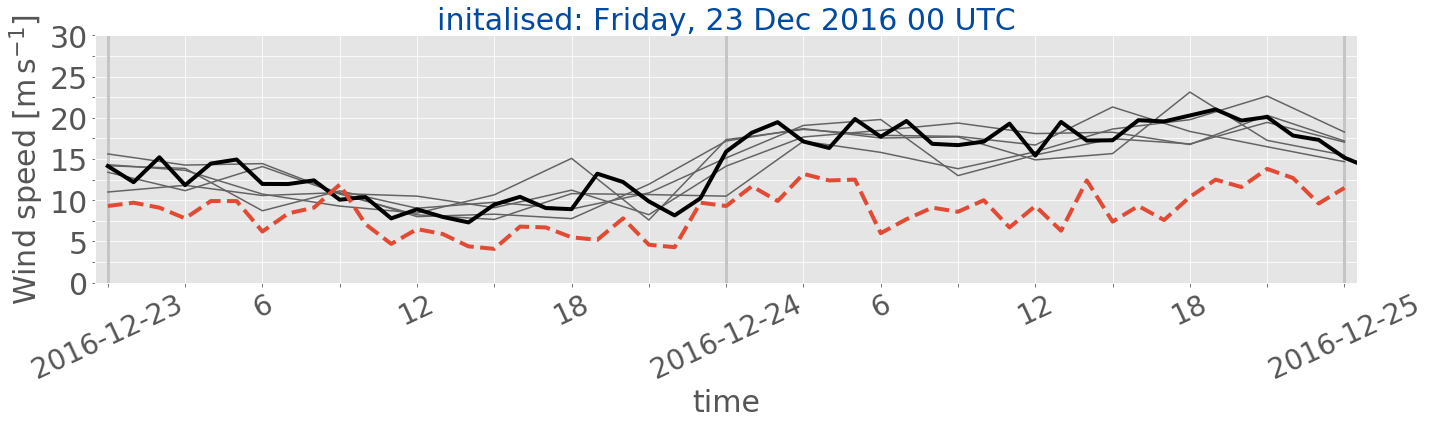
\includegraphics[trim={0.cm 5.cm 0cm 0cm},clip,
		width=\textwidth]{./fig_sfc_ws/20161223_00}
		\caption{}\label{fig:res:sfc_ws23}
	\end{subfigure}
	%
	\begin{subfigure}[b]{0.49\textwidth}
		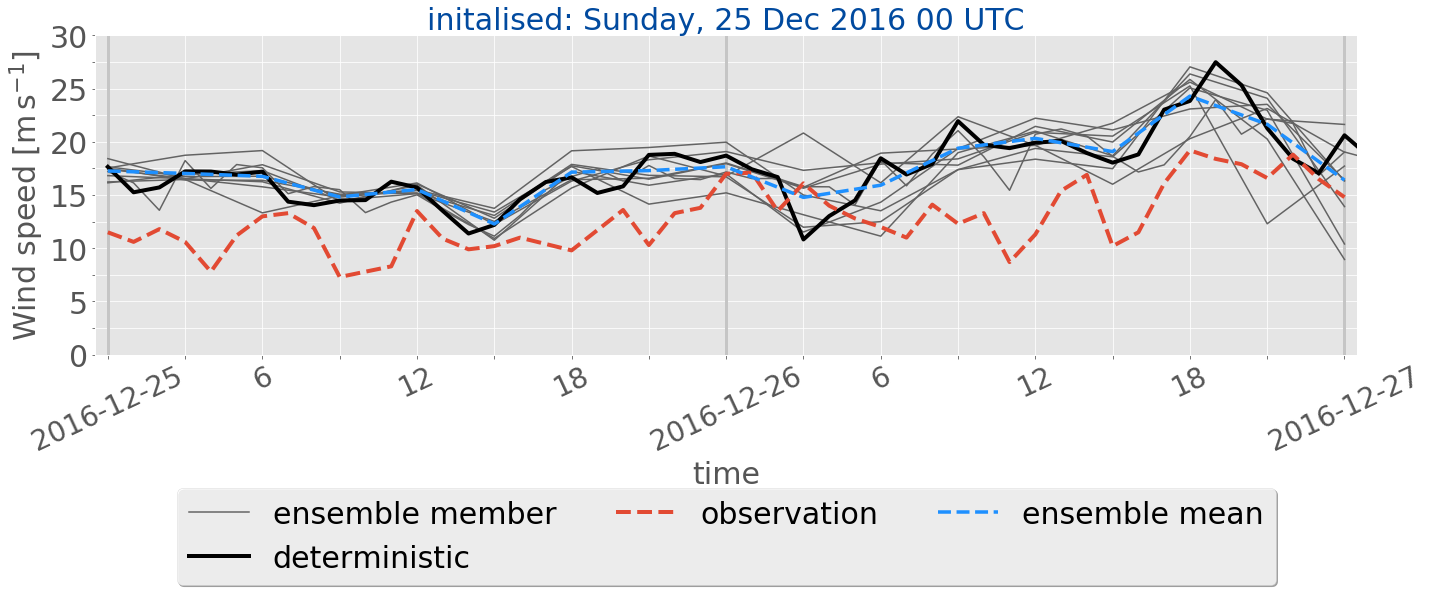
\includegraphics[trim={0.cm 5.cm 0cm 0cm},clip,
		width=\textwidth]{./fig_sfc_ws/20161225_00}
		\caption{}\label{fig:res:sfc_ws25}
	\end{subfigure}
	% sfc precip
	\begin{subfigure}[b]{0.49\textwidth}
		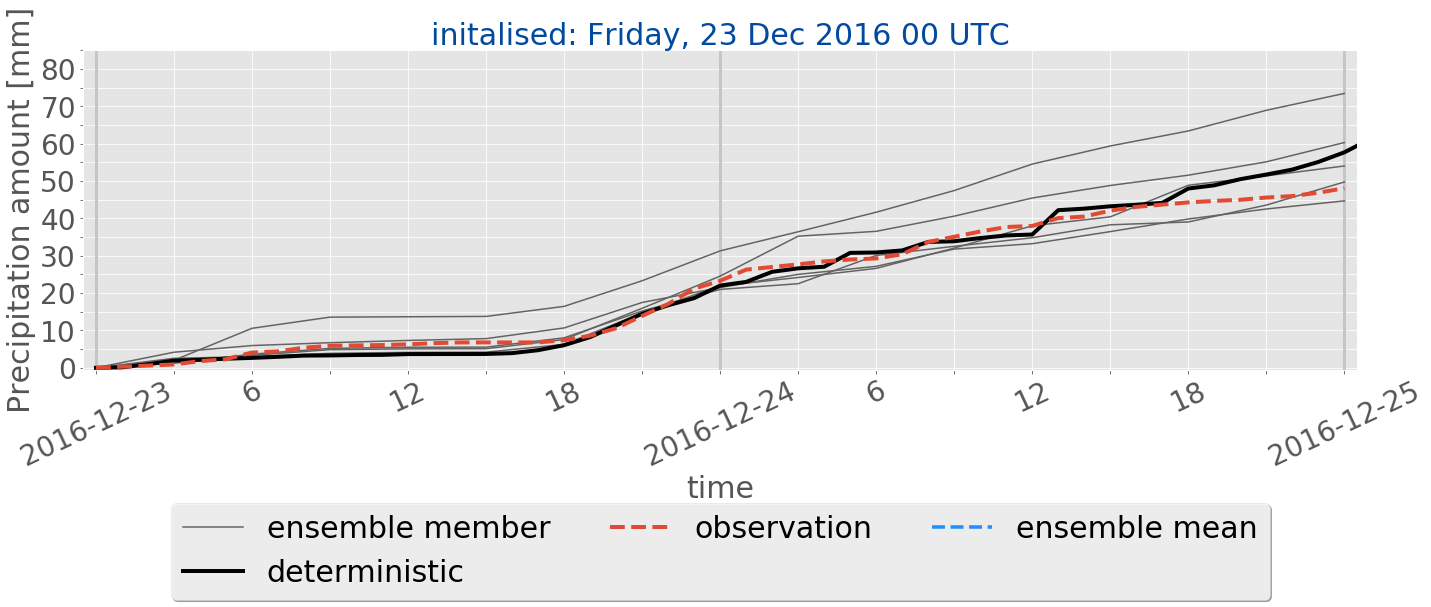
\includegraphics[trim={0.cm 3.6cm 0cm 0cm},clip,
		width=\textwidth]{./fig_sfc_precip/20161223_00}
		\caption{}\label{fig:res:sfc_precip23}
	\end{subfigure}
	%
	\begin{subfigure}[b]{0.49\textwidth}
		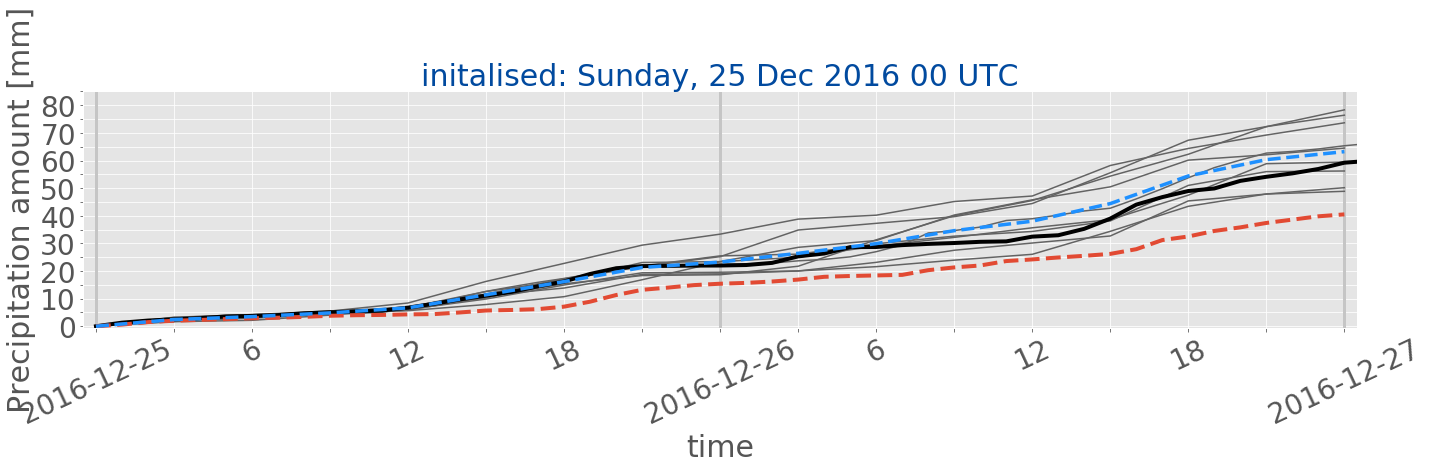
\includegraphics[trim={0.cm 3.6cm 0cm 0cm},clip,
		width=\textwidth]{./fig_sfc_precip/20161225_00}
		\caption{}\label{fig:res:sfc_precip25}
	\end{subfigure}
	
	% label
	\begin{subfigure}[b]{\textwidth}
		\centering
		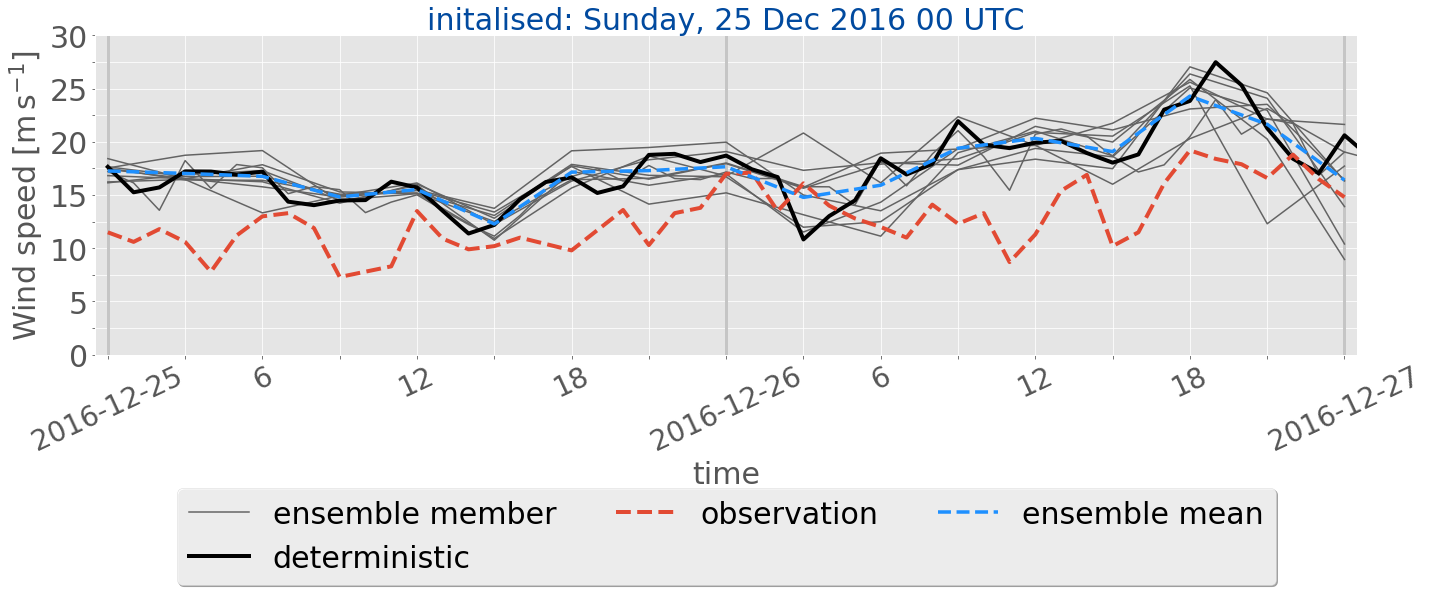
\includegraphics[trim={5.5cm 0cm 5.cm 17.2cm},clip,
		width=0.8\textwidth]{./fig_sfc_ws/20161225_00}
	\end{subfigure}
    \caption{\SI{48}{\hour} surface observations and ensemble forecasts initialised on the \SI{23}{\dec} at \SI{0}{\UTC} (left column, \protect\subref{fig:res:sfc_pres23}, \protect\subref{fig:res:sfc_temp23}, \protect\subref{fig:res:sfc_wd23}, \protect\subref{fig:res:sfc_ws23}, \protect\subref{fig:res:sfc_precip23}), and on \SI{25}{\dec} at \SI{0}{\UTC} (right column, \protect\subref{fig:res:sfc_pres25}, \protect\subref{fig:res:sfc_temp25}, \protect\subref{fig:res:sfc_wd25}, \protect\subref{fig:res:sfc_ws25}, \protect\subref{fig:res:sfc_precip25}) as well as \SI{26}{\dec} (\protect\subref{fig:res:sfc_pres26}, \protect\subref{fig:res:sfc_temp26}, \protect\subref{fig:res:sfc_wd26}, \protect\subref{fig:res:sfc_ws26}, \protect\subref{fig:res:sfc_precip26}). Line representation according to the label. Upper panel sea level pressure, second \SI{2}{\metre} air temperature, third and fourth \SI{10}{\metre} wind direction and speed, respectively, and lowest panel precipitation amount. }\label{fig:res:sfc_obs_meps}
	%
\end{figure}
\begin{figure}[H]\ContinuedFloat
	\centering
	% sfc pressure
	\begin{subfigure}[b]{0.49\textwidth}
		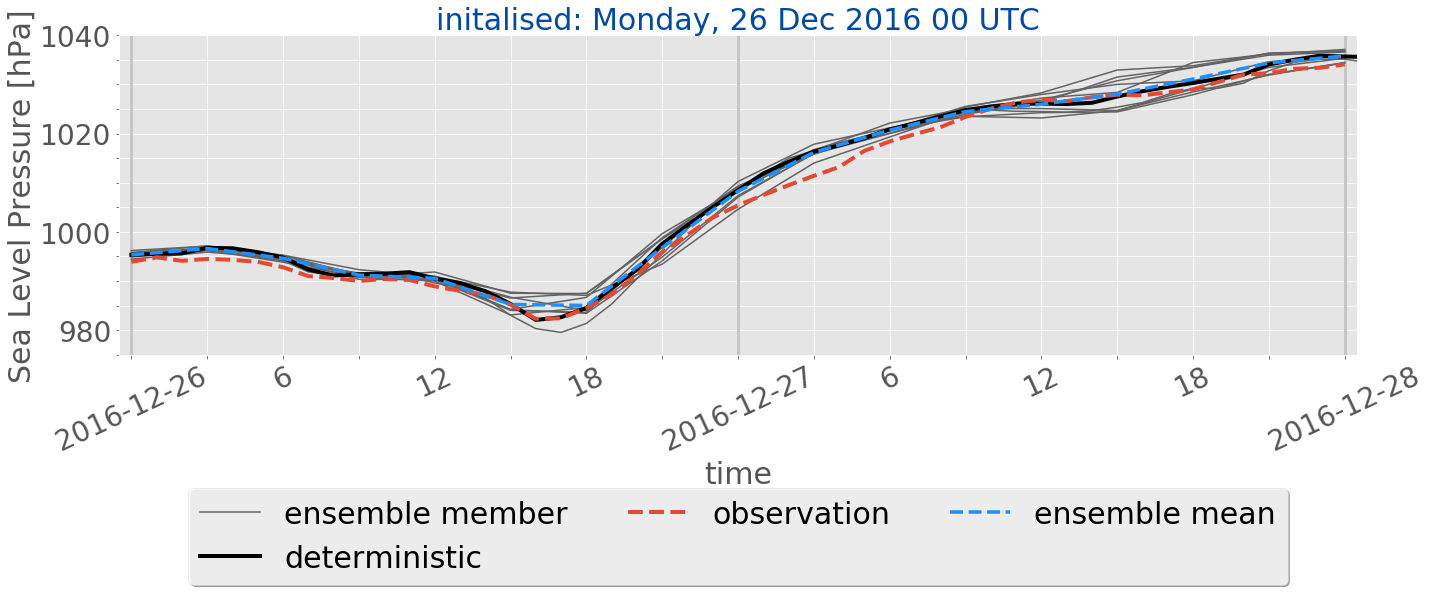
\includegraphics[trim={0.cm 5.cm 0cm 0cm},clip,
		width=\textwidth]{./fig_sfc_pressure/20161226_00}
		\caption{}\label{fig:res:sfc_pres26}
	\end{subfigure}
	
	% sfc temp
	\begin{subfigure}[b]{0.49\textwidth}
		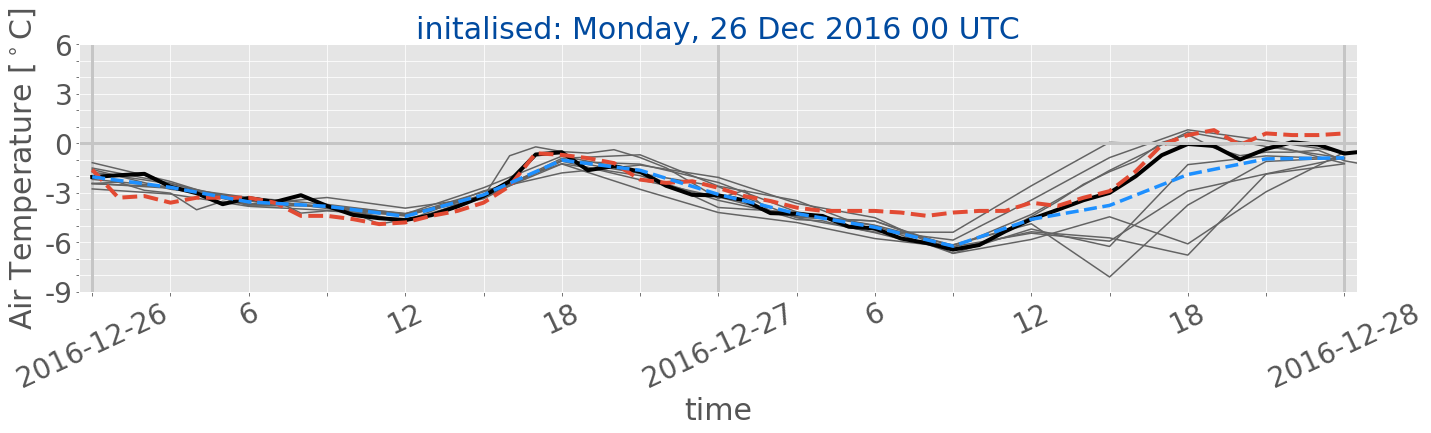
\includegraphics[trim={0.cm 5.cm 0cm 0cm},clip,
		width=\textwidth]{./fig_sfc_temp/20161226_00}
		\caption{}\label{fig:res:sfc_temp26}
	\end{subfigure}
	
	% sfc wd
	\begin{subfigure}[b]{0.49\textwidth}
		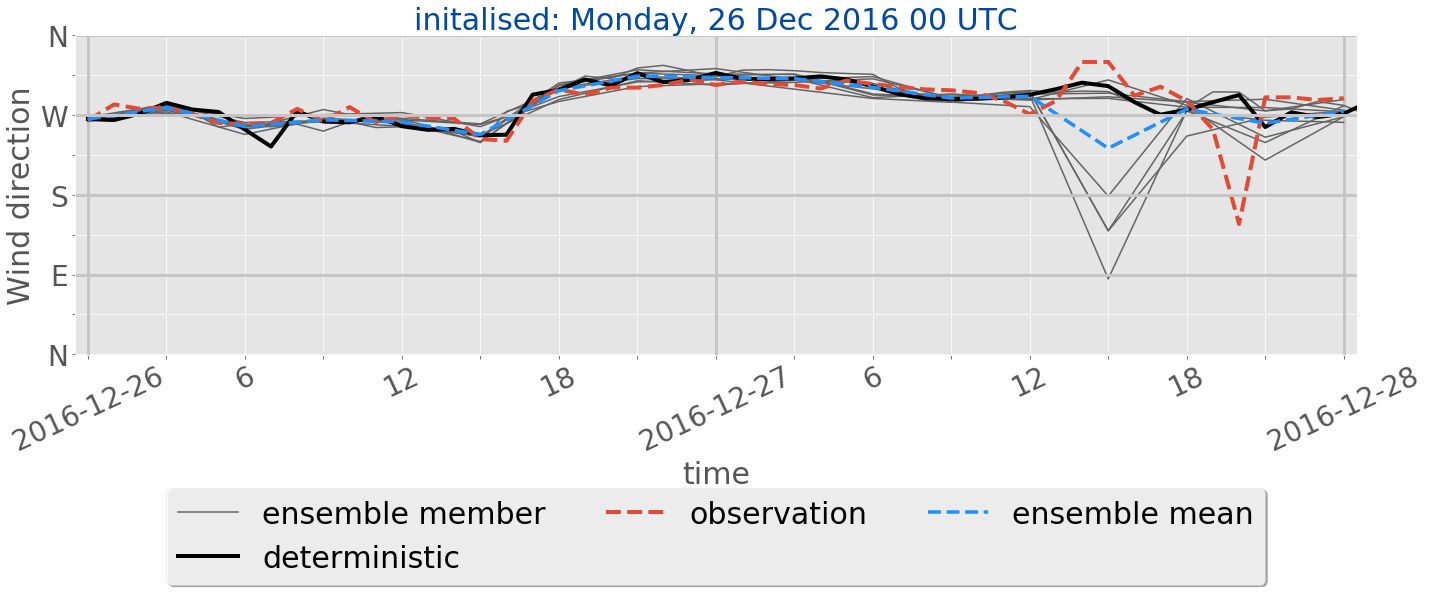
\includegraphics[trim={0.cm 5.cm 0cm 0cm},clip,
		width=\textwidth]{./fig_sfc_wd/20161226_00}
		\caption{}\label{fig:res:sfc_wd26}
	\end{subfigure}
	
	% sfc ws
	\begin{subfigure}[b]{0.49\textwidth}
		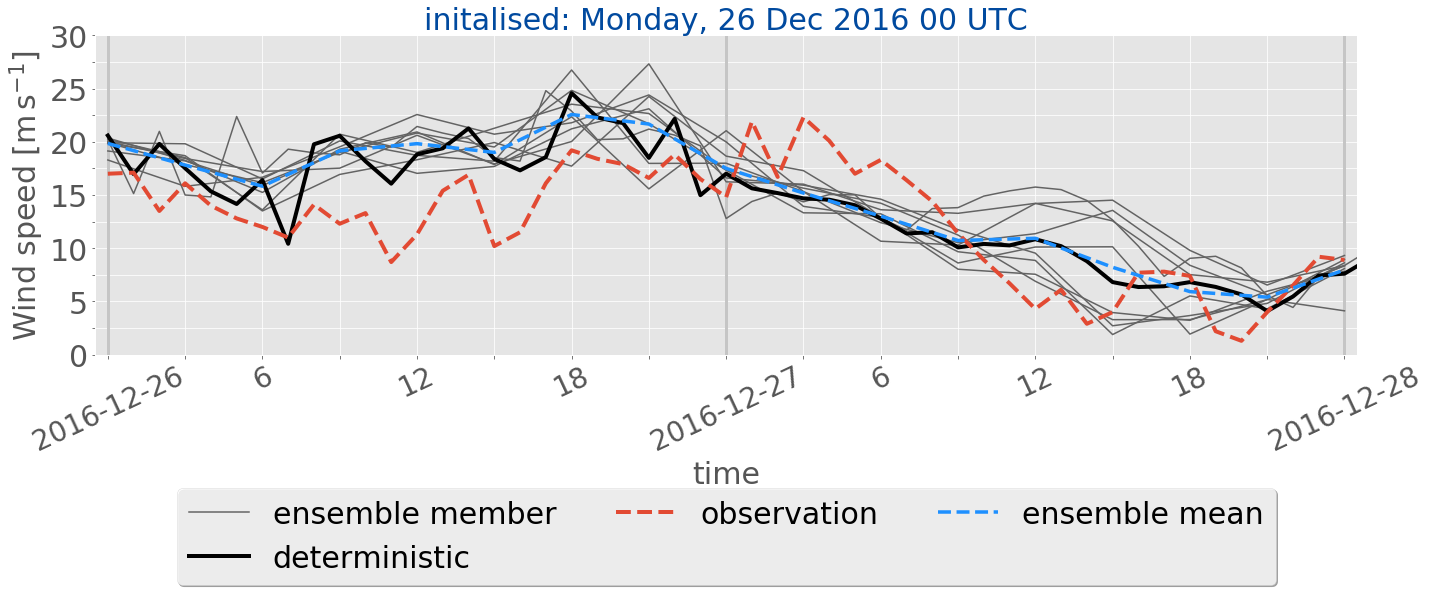
\includegraphics[trim={0.cm 5.cm 0cm 0cm},clip,
		width=\textwidth]{./fig_sfc_ws/20161226_00}
		\caption{}\label{fig:res:sfc_ws26}
	\end{subfigure}
	
	% sfc precip
	\begin{subfigure}[b]{0.49\textwidth}
		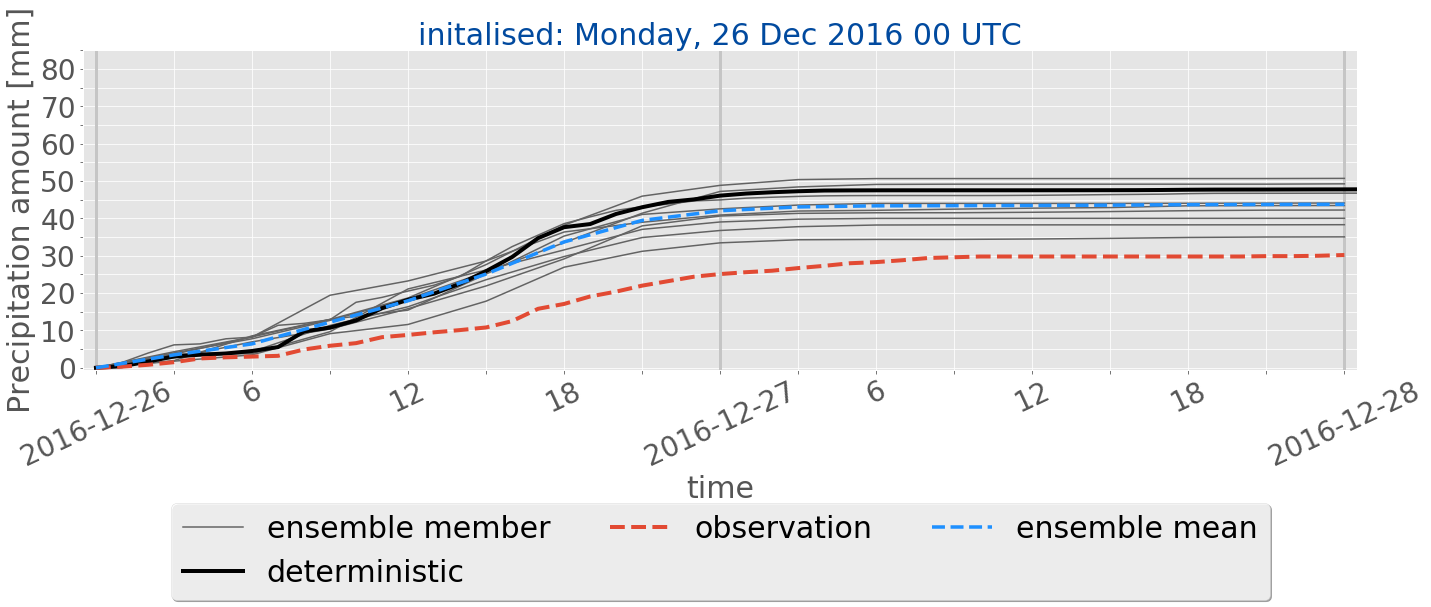
\includegraphics[trim={0.cm 3.6cm 0cm 0cm},clip,
		width=\textwidth]{./fig_sfc_precip/20161226_00}
		\caption{}\label{fig:res:sfc_precip26}
	\end{subfigure}
	
	% label
	\begin{subfigure}[b]{\textwidth}
		\centering
		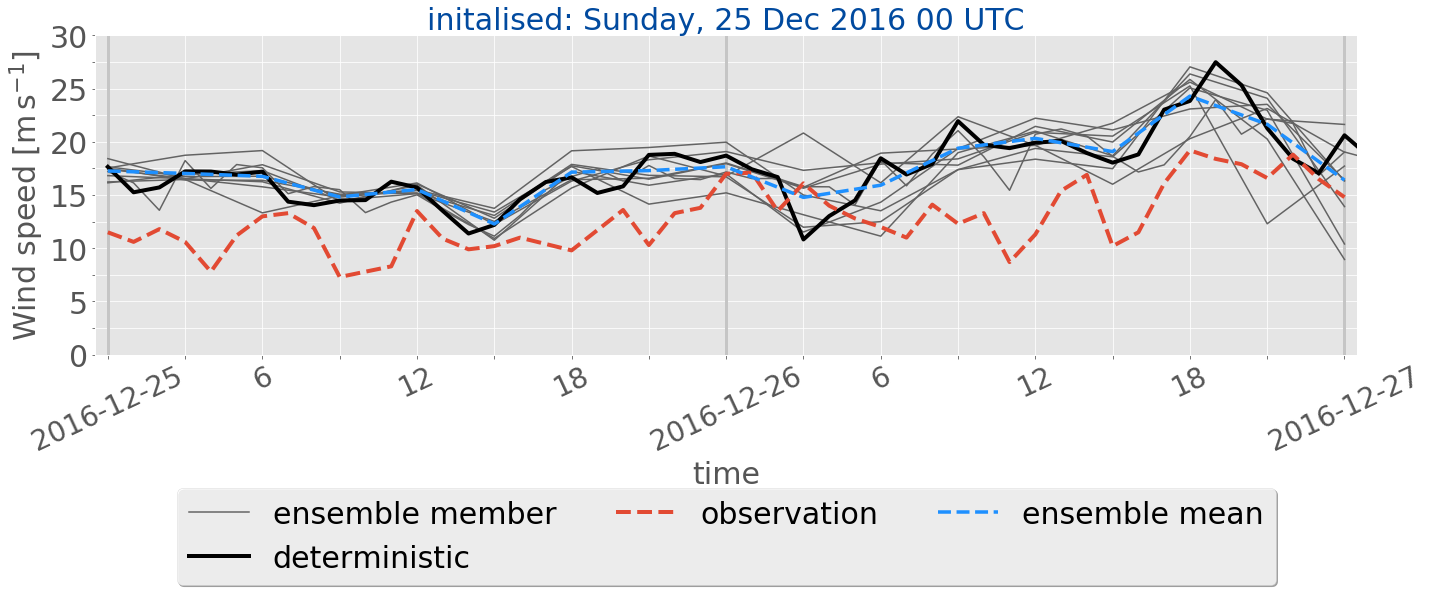
\includegraphics[trim={5.5cm 0cm 5.cm 17.2cm},clip,
		width=0.8\textwidth]{./fig_sfc_ws/20161225_00}
	\end{subfigure}
    \caption{\textit{(Continued from previous page.)} Initialisation \SI{26}{\dec} at \SI{0}{\UTC}.}
\end{figure}
%%%%%%%%%%%%%%%%%%%%%%%%%%%%%%%%%%%%%%%%%%%%%%
\pagebreak
\noindent
As described in \Cref{sec:largeScale} shows the ECMWF dynamic tropopause analysis map (\Cref{fig:DT23}) more ridging and therefore warmer air over Southern Norway on \SI{23}{\dec}. The low-pressure system approaches in the course of the day south-east of Iceland and hence stronger west to south west wind are associated with the cyclone (\Cref{fig:GP23}). The MEPS forecast, initialised on \SI{23}{\dec} at \SI{0}{\UTC} in \Cref{fig:res:sfc_pres23} follows the observations and shows the decrease in pressure after \SI{12}{\UTC} due to the passage of the occluded front with a constant pressure after the transition. Since warmer air is more advected to the north and the DT in \Cref{fig:DT23} shows a warm low-pressure core, an increase in temperature was observed and predicted at the measurement site (\Cref{fig:res:sfc_temp23}). 
\\
As the cyclone is advected to the north-east, closer into the Norwegian Sea, a wind change can be seen in the analysis map from ECMWF (\Cref{fig:GP23}). First west wind and later south-west wind was associated with the low-pressure system. The MEPS forecast and observations in \Cref{fig:res:sfc_wd23} and \subref{fig:res:sfc_ws23} indicate a wind change from west to south with a slight decrease in wind speed.
\\
On \SI{23}{\dec} was the passage of the occlusion also observed by an increase in precipitation. Before \SI{18}{\UTC} shows the surface accumulation light precipitation. During the passage of the occluded front increases the observed surface accumulation and is associated to continuous, heavy precipitation.
\\
\\
Similar patterns were seen for the passage of the occluded front on \SI{26}{\dec} in the ECMWF analysis \Cref{fig:DT26} and \ref{fig:GP26}. In this case the low-pressure system was located north of Morø og Romsdal in the Norwegian Sea. In the morning was the cyclone located east of Iceland and in the course of the day it got closer to the coast of Norway. Before landfall at \SI{16}{\UTC} indicates \Cref{fig:res:sfc_pres26} a pressure decrease. During the passage the sea level pressure reaches its lowest point of \SI{985}{\hPa} and increased afterwards during the dissipation of the Christmas storm. Pressure, temperature, and wind changes were already forecasted for initialisations on \SI{25}{\dec} (\Cref{fig:res:sfc_pres25}, \subref{fig:res:sfc_temp25}, \subref{fig:res:sfc_wd25}, \subref{fig:res:sfc_ws25}), only wind speed and precipitation seem not to agree with the observations at Haukeliseter.
\\
Since the cyclone was surrounded by colder air (south of the low-pressure system) first a drop and then an increase of temperature were observed and forecasted by MEPS. An indication of the passage is also seen in the \SI{10}{\metre} wind observations and forecasts. As the cyclone is east of Iceland with a westward large-scale surface wind (\Cref{fig:GP26_00} and \Cref{fig:GP26_12}), shows \Cref{fig:res:sfc_wd26} and \subref{fig:res:sfc_ws26} west wind with observed strength up to \SI{17.5}{\mPs}. During the passage changes the wind direction to north-west with higher wind speed which can be associated to the location of the low-pressure system and the closer surface isobars (\Cref{fig:DT26}). 
\\
The precipitation was continuing throughout the day, with light to moderate precipitation before the passage and heavy precipitation around \SI{16}{\UTC} followed by moderate to light precipitation. 
\\
%%%%%%% image liquid obs particle %%%%%%%%%%%%%%%%
\begin{figure}[t]
	\centering
	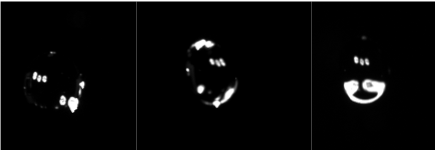
\includegraphics[%trim={45.cm 30.cm 13cm 35cm},clip,
	width=0.8\textwidth]{./MASC_obs/Masc_obs_liquid_2512}
	\caption{MASC images of falling water drops observed on \SI{25}{\dec} at \SI{17}{\UTC} from three different angles. Not all parts of the liquid sphere are equally illuminated.}\label{fig:res:obs_masc}
\end{figure}
%%%%%%%%%%%%%%%%%%%%%%%%%%%%%%%%%%%%%%%%%%%%%%
\\
While on \SIlist{23;25}{\dec} the precipitation was associated with a passage/landfall of an occluded front, was the \SI{25}{\dec} marked by the transition of a warm sector. The ECMWF analysis showed a ridging at the DT surface. The surface cyclone core is south east of Iceland in \Cref{fig:DT25} with two associated frontal boundaries. While the warm front is approaching the west coast, is the cold front north-west of Great Britain. The cold fronts tail moved into lower latitudes, following the slowdown of the cold front, leading to a stationary frontal boundary. Furthermore, the mid-latitude jet is aligned along the surface frontal boundaries (\Cref{fig:DT25_00}), while the Haukeliseter site is located below the left jet exit region. This leads to rising motion at the surface.
\\
Neither pressure nor wind observations and forecasts indicate the passage of any frontal boundary. The only indication of the transition is seen in the increase of temperature at \SI{11}{\UTC} until \SI{21}{\UTC} (\Cref{fig:res:sfc_temp25}). In \Cref{fig:res:sfc_wd25} a small wind change was observed by the wind mast at \SI{10}{\UTC}. This development from west to north-west was not forecasted by MEPS, it rather estimated strong west winds.
\\
In \Cref{fig:res:obs_masc} are the surface observations from the MASC during the passage of the warm sector. Without the images taken around \SI{17}{\UTC} it would not be possible to verify that liquid precipitation occurred at the Haukeliseter site. Together with the increase in surface temperature in \Cref{fig:res:sfc_temp25} it is qualified that at least the warm sector of the low-pressure system appeared at the measurement site.
\textcolor{red}{Should I include the DIANA analysis maps? But I dont know what the meteorologists are using to produce them? ECMWF?}
%
%%%%%%% image scatter obs ret %%%%%%%%%%%%%%%%
\begin{figure}[t!]
	\centering
	% sfc pressure
	\begin{subfigure}[b]{0.49\textwidth}
		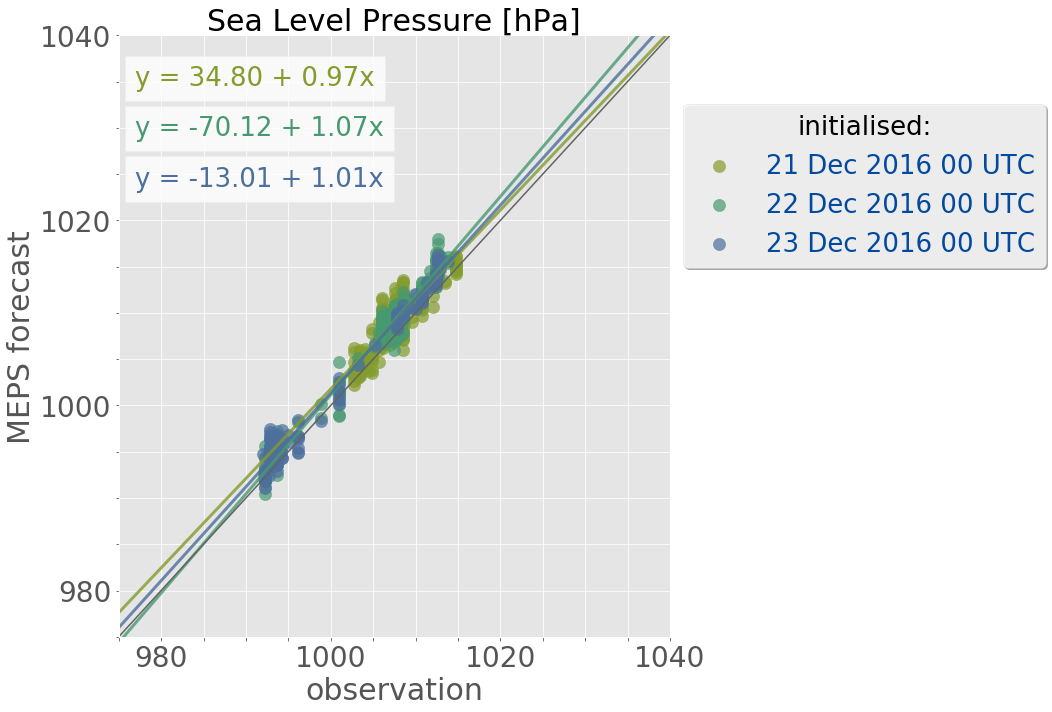
\includegraphics[trim={0.cm 0cm 12.5cm 0cm},clip,
		width=\textwidth]{./fig_sfc_pressure/obs_model_20161221_23_00}
		\caption{}\label{fig:scat:pres2123}
	\end{subfigure}
	%
	\begin{subfigure}[b]{0.49\textwidth}
		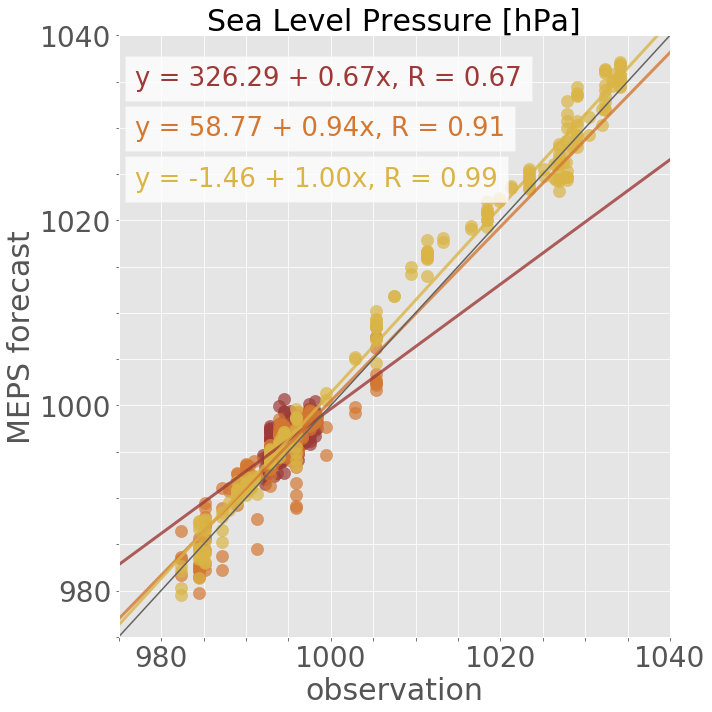
\includegraphics[trim={0.cm 0cm 12.5cm 0cm},clip,
		width=\textwidth]{./fig_sfc_pressure/obs_model_20161224_26_00}
		\caption{}\label{fig:scat:pres2426}
	\end{subfigure}
    \caption{\SI{48}{\hour} scatter plots for surface observations and ensemble forecasts initialised for \SIrange{21}{23}{\dec} (left column, \protect\subref{fig:scat:pres2123}, \protect\subref{fig:scat:temp2123}, \protect\subref{fig:scat:wd2123}, \protect\subref{fig:scat:ws2123}, \protect\subref{fig:scat:precip2123}) and  for \SIrange{24}{26}{\dec} (right column, \protect\subref{fig:scat:pres2426}, \protect\subref{fig:scat:temp2426}, \protect\subref{fig:scat:wd2426}, \protect\subref{fig:scat:ws2426}, \protect\subref{fig:scat:precip2426}). Sea level pressure.}\label{fig:scat:obs_meps}
\end{figure}
\begin{figure}\ContinuedFloat
	\centering
    %     % sfc temp
	\begin{subfigure}[b]{0.49\textwidth}
		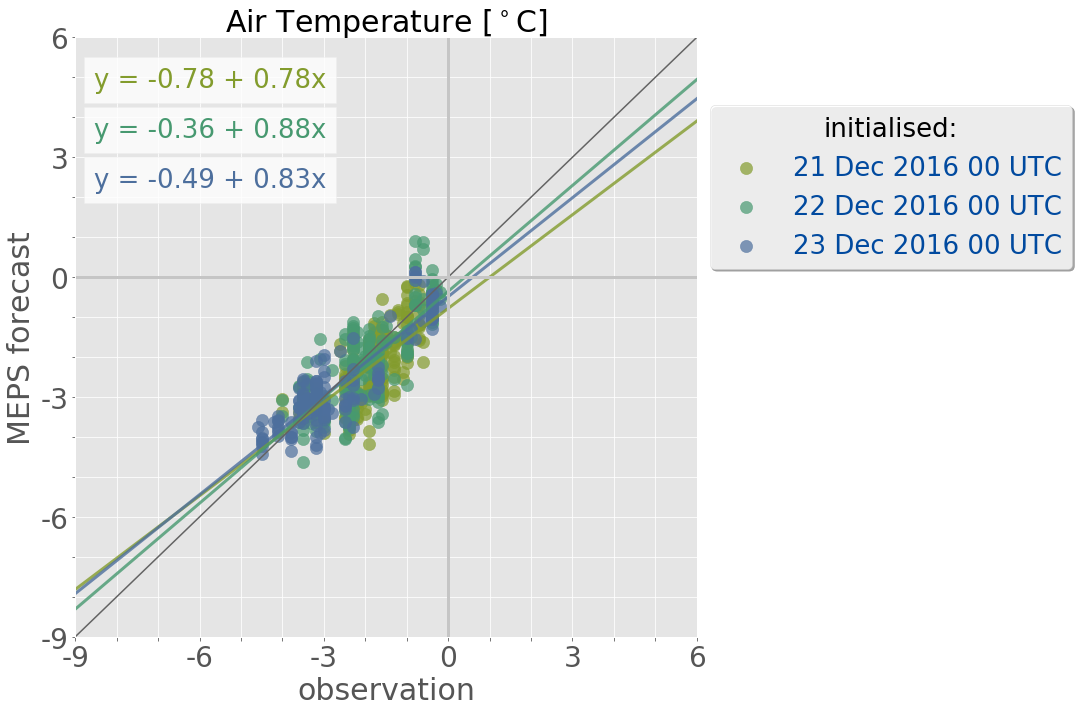
\includegraphics[trim={0.cm 0cm 12.5cm 0cm},clip,
		width=\textwidth]{./fig_sfc_temp/obs_model_20161221_23_00}
		\caption{}\label{fig:scat:temp2123}
	\end{subfigure}
	%
	\begin{subfigure}[b]{0.49\textwidth}
		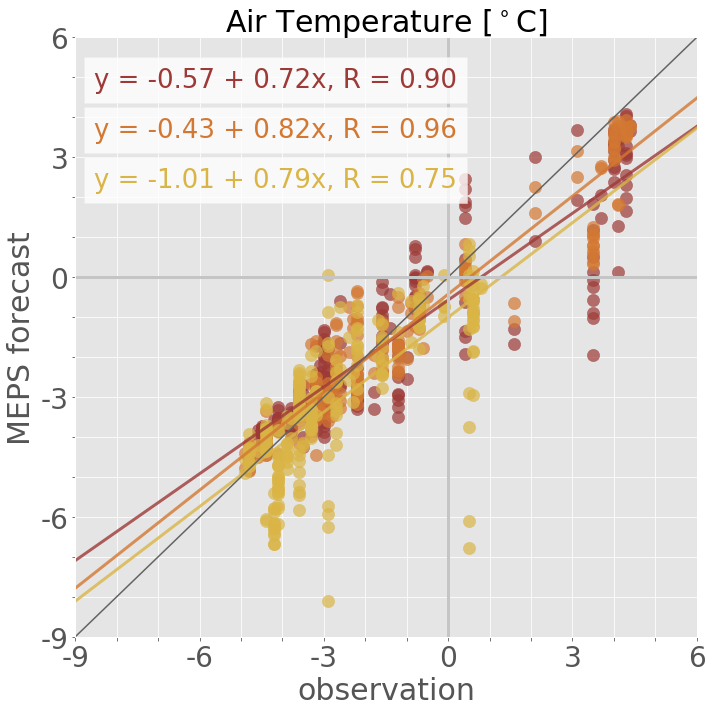
\includegraphics[trim={0.cm 0cm 12.5cm 0cm},clip,
		width=\textwidth]{./fig_sfc_temp/obs_model_20161224_26_00}
		\caption{}\label{fig:scat:temp2426}
	\end{subfigure}
% 	
% 	% label
% 	\begin{subfigure}[b]{0.49\textwidth}
% 		\centering
% 		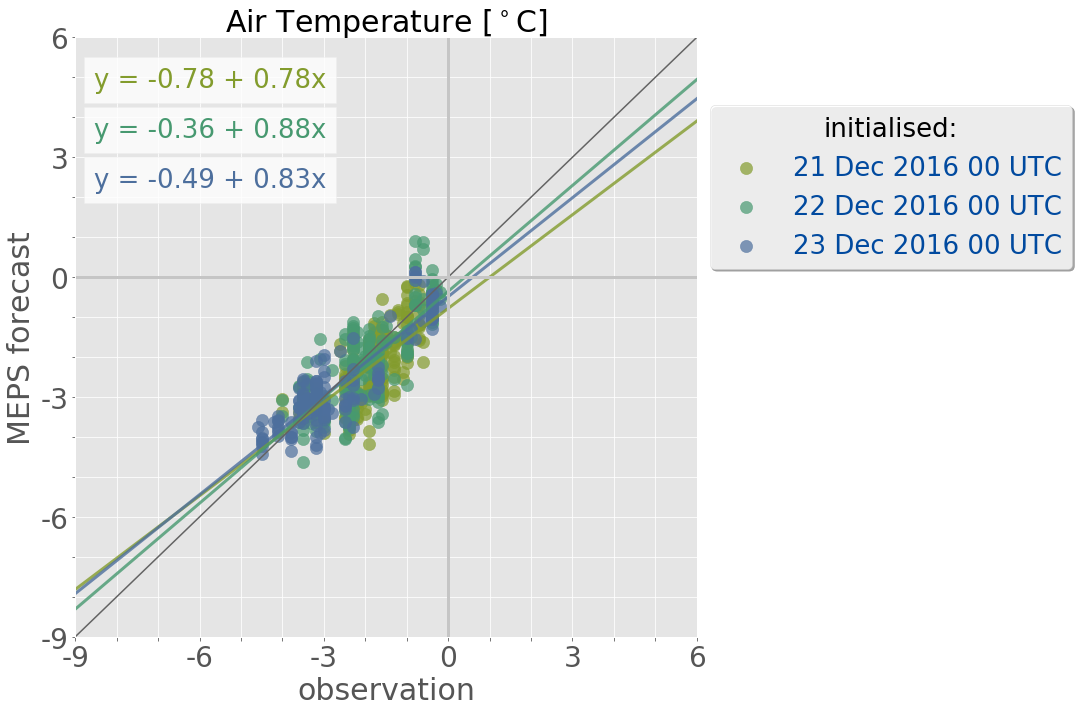
\includegraphics[trim={25.cm 15.5cm 0cm 3.6cm},clip,
% 		width=0.8\textwidth]{./fig_sfc_temp/obs_model_20161221_23_00}
% 	\end{subfigure}
% 	\begin{subfigure}[b]{0.49\textwidth}
% 		\centering
% 		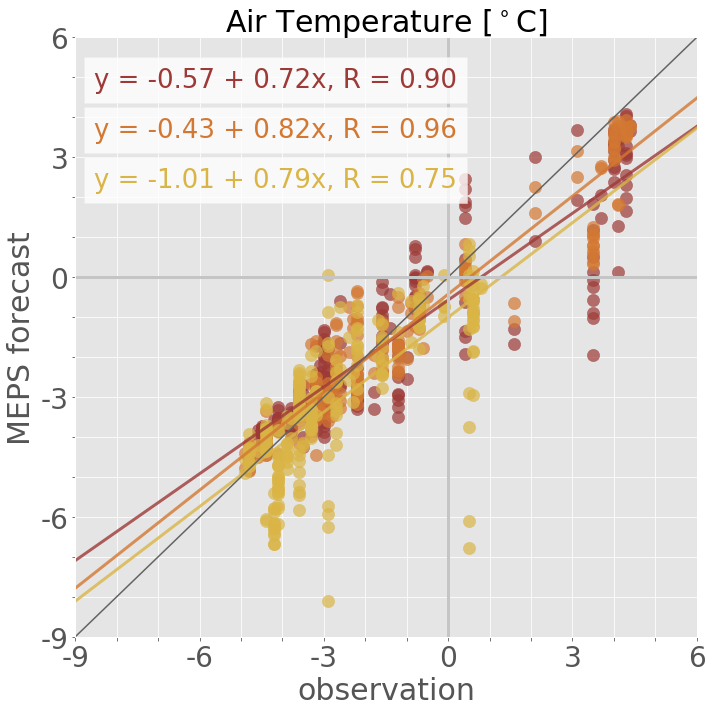
\includegraphics[trim={25.cm 15.5cm 0cm 3.6cm},clip,
% 		width=0.8\textwidth]{./fig_sfc_temp/obs_model_20161224_26_00}
% 	\end{subfigure}
% \end{figure}
% \begin{figure}\ContinuedFloat
	% sfc wd
	\begin{subfigure}[b]{0.49\textwidth}
		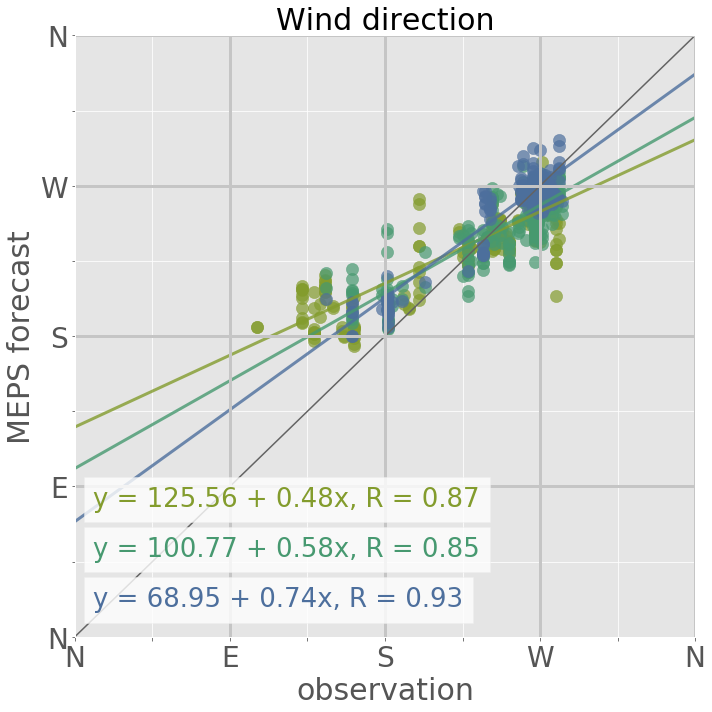
\includegraphics[trim={0.cm 0cm 12.5cm 0cm},clip,
		width=\textwidth]{./fig_sfc_wd/obs_model_20161221_23_00}
		\caption{}\label{fig:scat:wd2123}
	\end{subfigure}
	%
	\begin{subfigure}[b]{0.49\textwidth}
		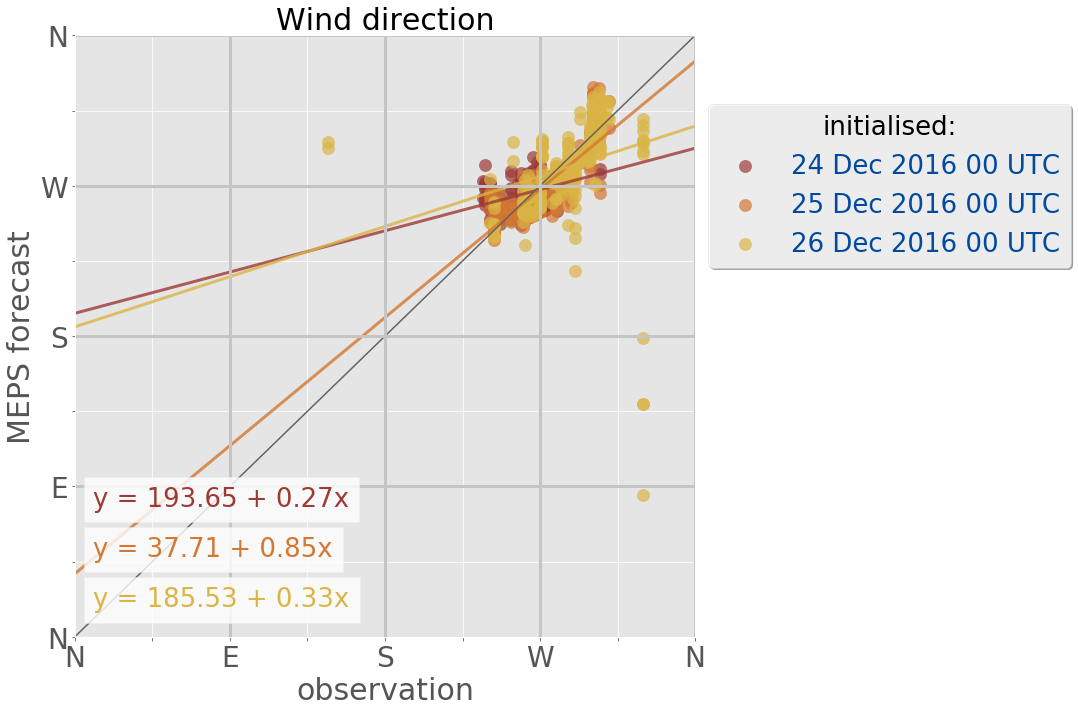
\includegraphics[trim={0.cm 0cm 12.5cm 0cm},clip,
		width=\textwidth]{./fig_sfc_wd/obs_model_20161224_26_00}
		\caption{}\label{fig:scat:wd2426}
	\end{subfigure}
    	
	% label
	\begin{subfigure}[b]{0.49\textwidth}
		\centering
		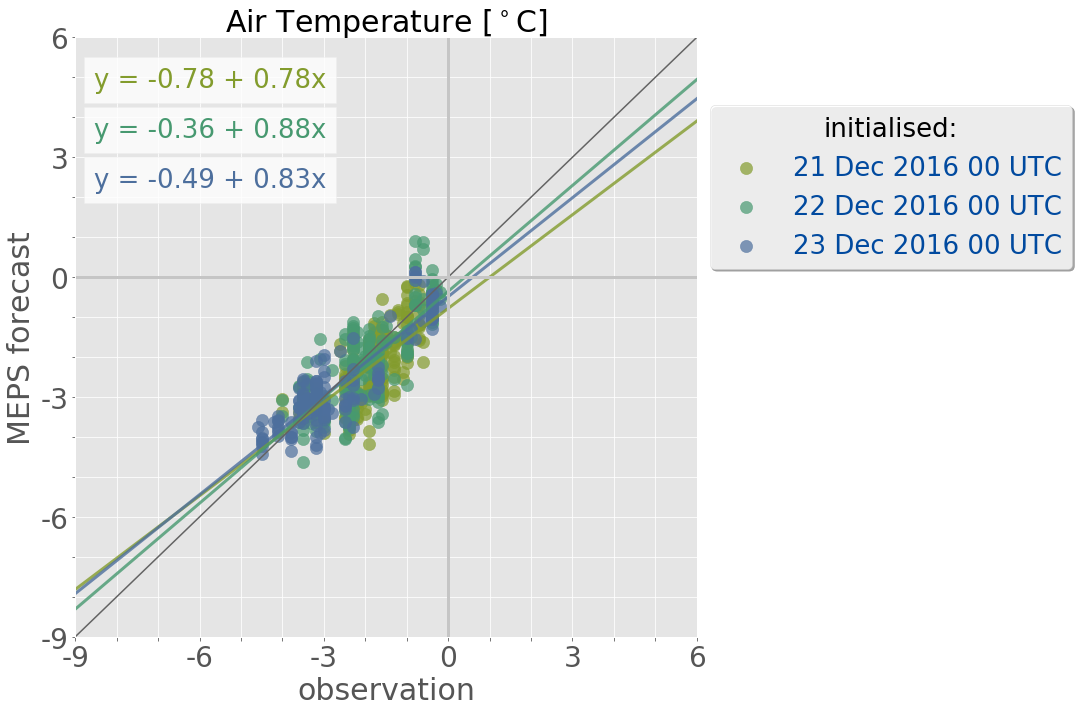
\includegraphics[trim={25.cm 15.5cm 0cm 3.6cm},clip,
		width=0.8\textwidth]{./fig_sfc_temp/obs_model_20161221_23_00}
	\end{subfigure}
	\begin{subfigure}[b]{0.49\textwidth}
		\centering
		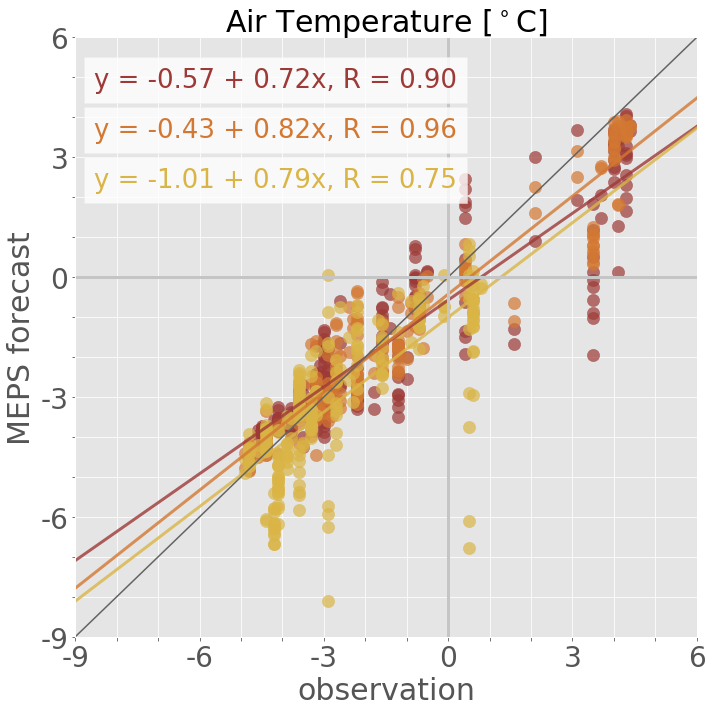
\includegraphics[trim={25.cm 15.5cm 0cm 3.6cm},clip,
		width=0.8\textwidth]{./fig_sfc_temp/obs_model_20161224_26_00}
	\end{subfigure}
    \caption{\textit{(Continued from previous page.)} Upper panel \SI{2}{\metre} air temperature, second panel \SI{10}{\metre} wind direction.}
\end{figure}
\begin{figure}\ContinuedFloat
	% sfc ws
	\begin{subfigure}[b]{0.49\textwidth}
		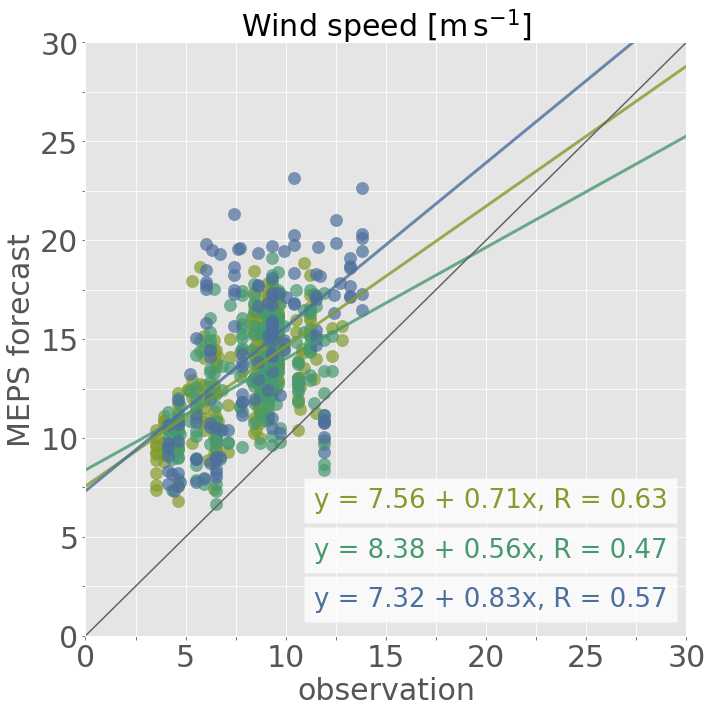
\includegraphics[trim={0.cm 0cm 12.5cm 0cm},clip,
		width=\textwidth]{./fig_sfc_ws/obs_model_20161221_23_00}
		\caption{}\label{fig:scat:ws2123}
	\end{subfigure}
	%
	\begin{subfigure}[b]{0.49\textwidth}
		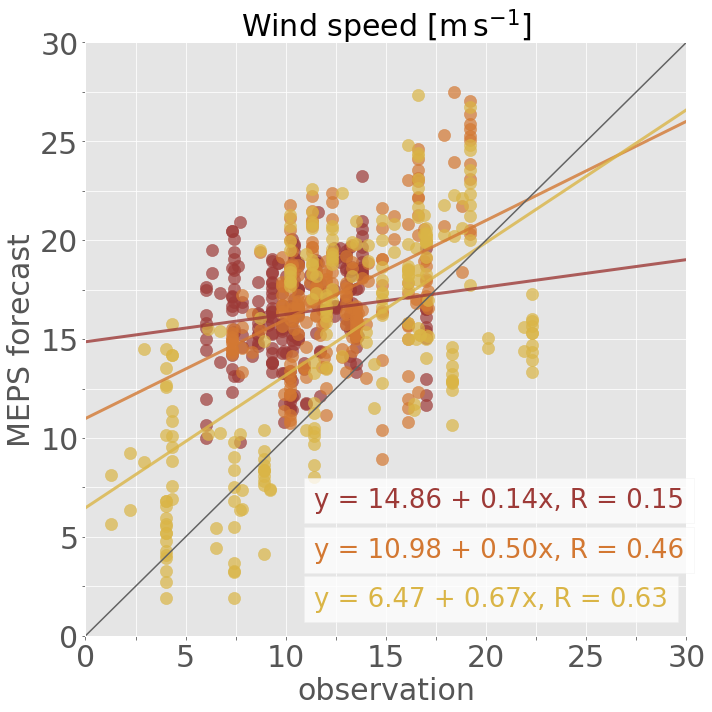
\includegraphics[trim={0.cm 0cm 12.5cm 0cm},clip,
		width=\textwidth]{./fig_sfc_ws/obs_model_20161224_26_00}
		\caption{}\label{fig:scat:ws2426}
	\end{subfigure}
% 	% label
% 	\begin{subfigure}[b]{0.49\textwidth}
% 		\centering
% 		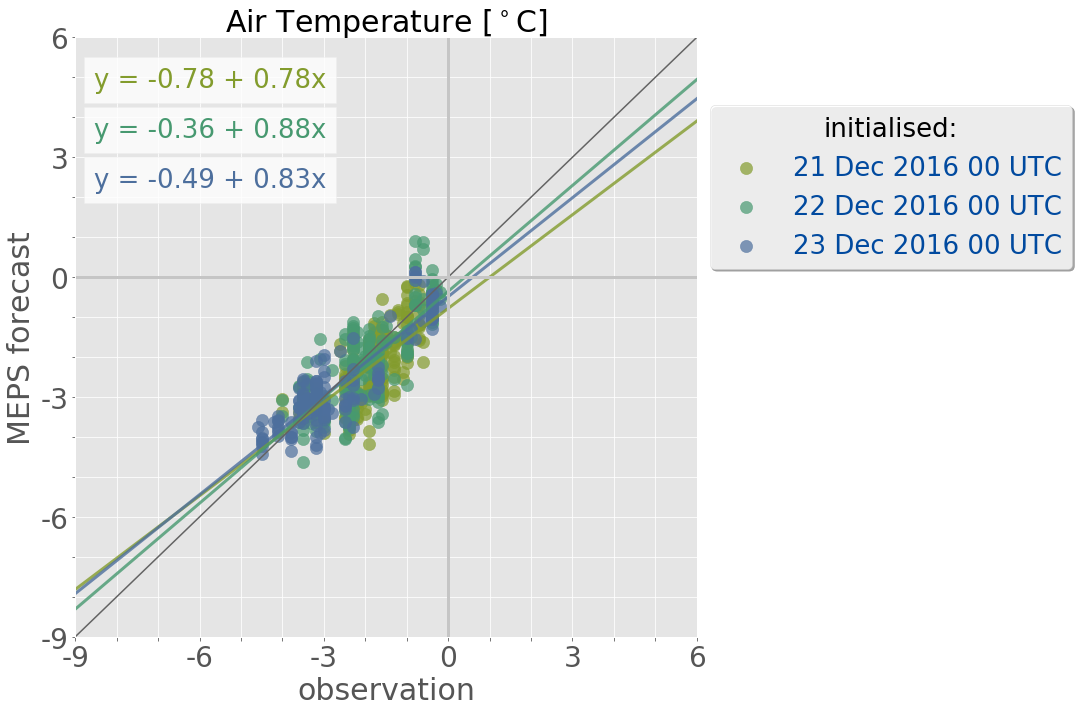
\includegraphics[trim={25.cm 15.5cm 0cm 3.6cm},clip,
% 		width=0.8\textwidth]{./fig_sfc_temp/obs_model_20161221_23_00}
% 	\end{subfigure}
% 	\begin{subfigure}[b]{0.49\textwidth}
% 		\centering
% 		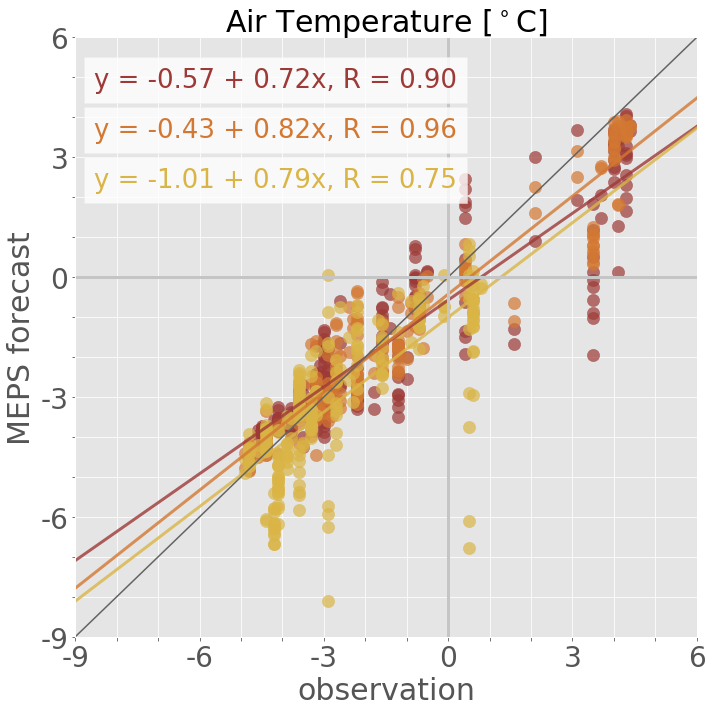
\includegraphics[trim={25.cm 15.5cm 0cm 3.6cm},clip,
% 		width=0.8\textwidth]{./fig_sfc_temp/obs_model_20161224_26_00}
% 	\end{subfigure}
%     \caption{\textit{(Continued from previous page.)} }
% \end{figure}
% \begin{figure}\ContinuedFloat
	% sfc precip
	\begin{subfigure}[b]{0.49\textwidth}
		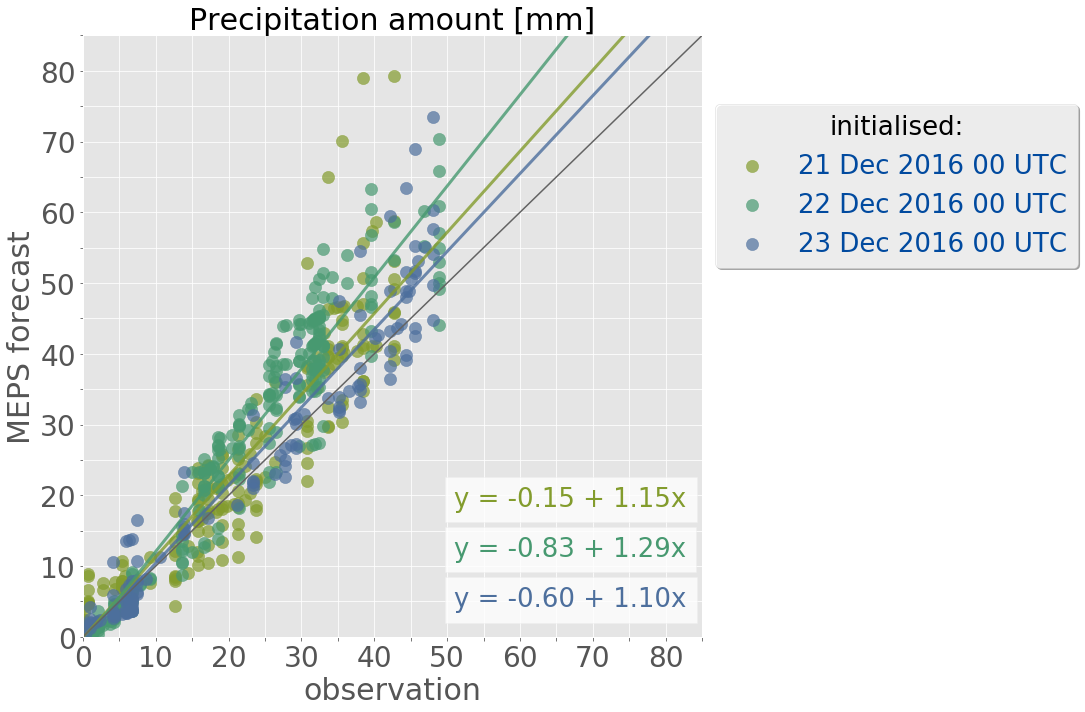
\includegraphics[trim={0.cm 0cm 12.5cm 0cm},clip,
		width=\textwidth]{./fig_sfc_precip/obs_model_20161221_23_00}
		\caption{}\label{fig:scat:precip2123}
	\end{subfigure}
	%
	\begin{subfigure}[b]{0.49\textwidth}
		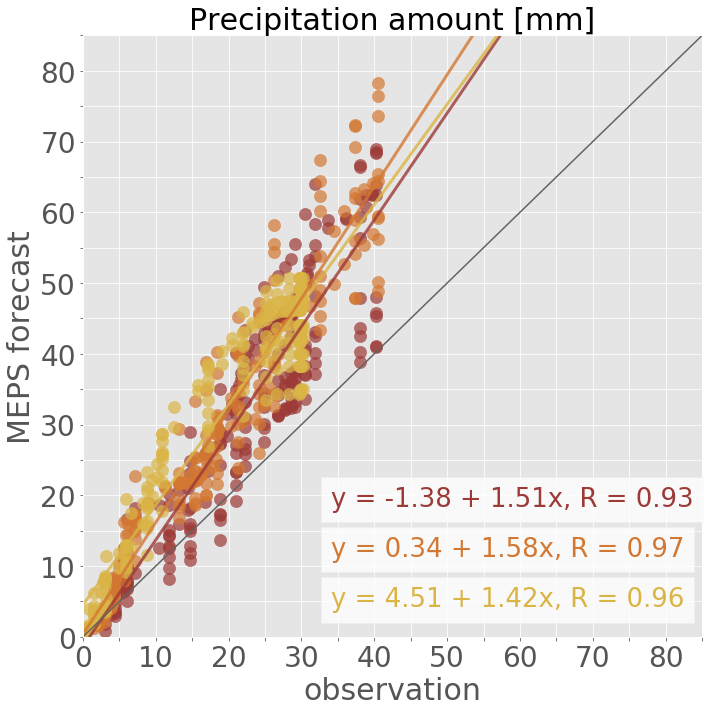
\includegraphics[trim={0.cm 0cm 12.5cm 0cm},clip,
		width=\textwidth]{./fig_sfc_precip/obs_model_20161224_26_00}
		\caption{}\label{fig:scat:precip2426}
	\end{subfigure}
	% label
	\begin{subfigure}[b]{0.49\textwidth}
		\centering
		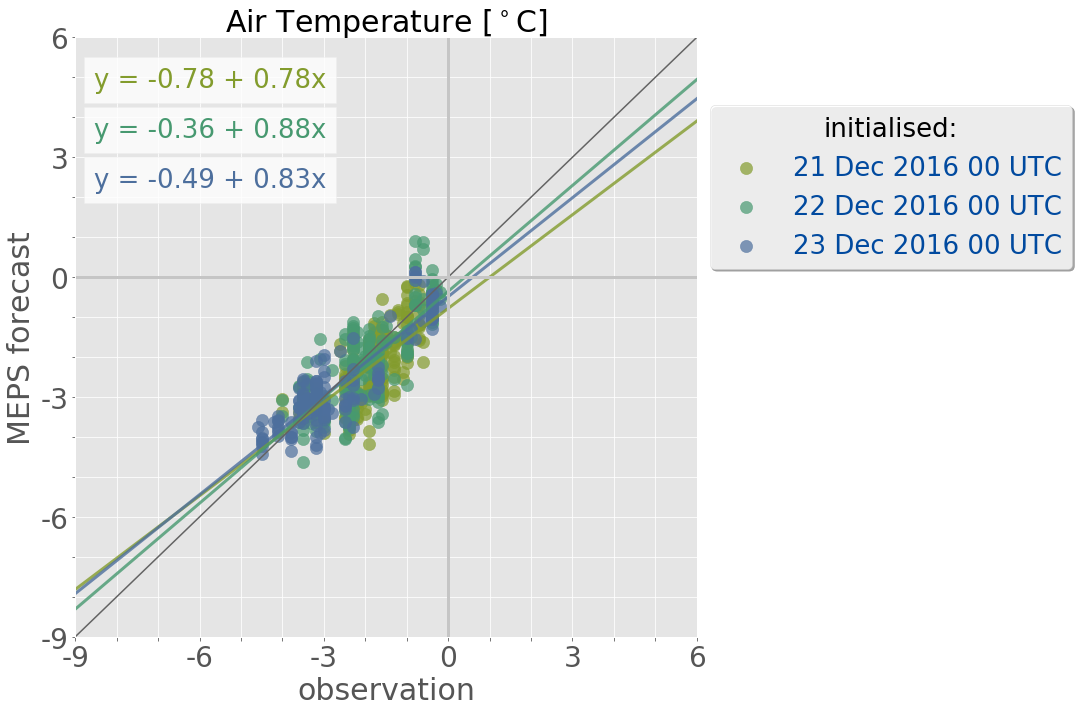
\includegraphics[trim={25.cm 15.5cm 0cm 3.6cm},clip,
		width=0.8\textwidth]{./fig_sfc_temp/obs_model_20161221_23_00}
	\end{subfigure}
	\begin{subfigure}[b]{0.49\textwidth}
		\centering
		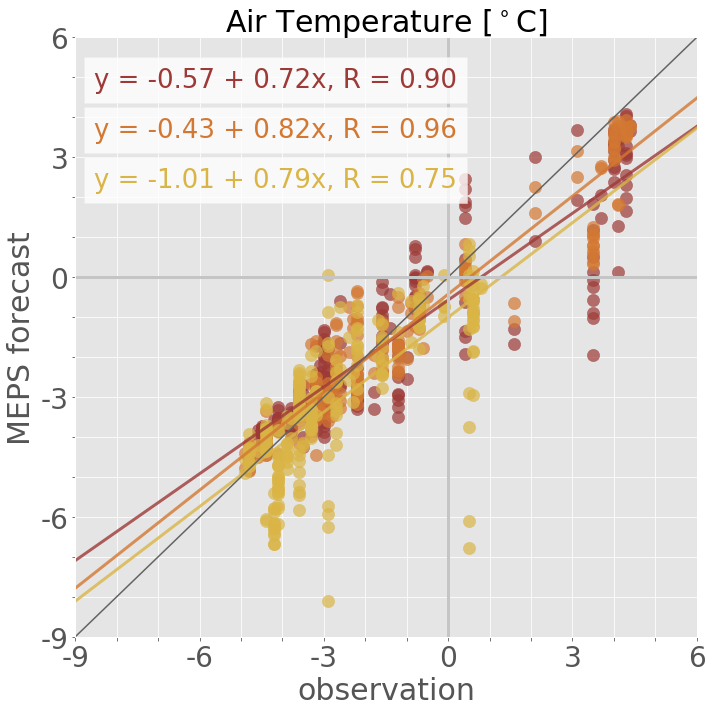
\includegraphics[trim={25.cm 15.5cm 0cm 3.6cm},clip,
		width=0.8\textwidth]{./fig_sfc_temp/obs_model_20161224_26_00}
	\end{subfigure}
	\caption{\textit{(Continued from previous page.)} Upper panel \SI{10}{\metre} wind speed, lower panel surface precipitation amount. }
\end{figure}
%%%%%%%%%%%%%%%%%%%%%%%%%%%%%%%%%%%%%%%%%%%%%%
\\
\\
The comparison between the ECMWF analysis displays, that the ensemble member forecast system MEPS covers the prediction of large scale phenomena like frontal boundaries and liquid precipitation at the surface. \Cref{fig:scat:obs_meps} presents the correlation between the observations and the \SI{48}{\hour} ensemble forecast. The relation between Haukeliseter observations and the forecast members is indicated by the regression line for each day.
\\
Sea level pressure has the best correlation under all variables. The best agreement shows on \SI{26}{\dec} when the Christmas storm made landfall and dissipates after the passage of the occluded front at \SI{16}{\UTC}. \citet{dahlgren_comparison_2013} showed that by mixing in large scale information from the boundary condition (ECMWF) into the regional model, the forecast for sea level pressure will be improved. The model-observation comparison by \citet{dahlgren_comparison_2013} showed a declination of forecasts with pressure mixing after \SI{24}{\hour} 
Since the pressure values are in good agreement with the observations is assumed that the warm front did not pass through at Haukeliseter on \SI{25}{\dec} and only the warm sector is observed. This shows a quite detailed forecast ability of MEPS, as from the ECMWF analysis it is not quite clear where the warm front could have passed through. 
\\
\Cref{fig:scat:temp2426} indicates a moderate correlation between observation and the \SI{48}{\hour} ensemble member forecast system. In general, underestimated MEPS the observed temperature, but it estimated it at the correct timing on \SI{25}{\dec}. The previous operational model AROME-MetCoOp showed a negative winter bias after winter 2012 \citep{muller_arome-metcoop:_2017}. \Cref{fig:bias:temp} shows for \SIlist{23;26}{\dec} positive as well as negative mean error for the individual members. On \SI{25}{\dec}, during the warm sector a negative bias was observed, underestimating the temperature when compared to the observation. The mean error for the Norwegian model domain of AROME-MetCoOP estimated by \citet{muller_arome-metcoop:_2017} is smaller than \SI{1.8}{\kelvin} for the surface temperature in December 2014. The forecasts for \SIlist{23;25;26}{\dec} show mean absolute error values of up to \SIlist{0.61;0.77;1.44}{\kelvin}, respectively. It shows by using an ensemble forecast system a reduction of mean errors and an increase in forecast accuracy can be done. 
\\
During the Christmas storm 2016 high wind speeds were observed at the Haukeliseter site (\Cref{fig:scat:ws2123} and \subref{fig:scat:ws2426}).
According to \citet{muller_arome-metcoop:_2017} are large wind speeds significantly better simulated for AROME-MetCoOp compared to ECMWF's forecast. The wind speeds are still overestimated, which is an already known difficulty in the deterministic version of MEPS. In AROME-MetCoOp wind speed prediction agreed better with observations for wind speeds between \SIrange{3}{13}{\mPs} than ECMWF forecasts did, showing the advantage of a high-resolution weather model. With increasing wind speed the forecast accuracy decreases with a mean absolute error below \SI{2}{\mPs} for December 2014 in AROME-MetCoOp.
The mean absolute error for wind speed during the Christmas storm is higher at all days ranging from \SIrange{3}{7}{\mPs}.
During the three days with frontal passages shows the \SI{23}{\dec} the highest mean absolute error of \SI{6.5}{\mPs}, more than three times as high as the monthly averaged value from \citet{muller_arome-metcoop:_2017}. Their study case in February 2015 showed a slight overestimation of ECMWF \SI{10}{\metre} wind compared to the Norwegian AROME-MetCoOp domain, but still overestimates MEPS the wind.
\textcolor{red}{What could be still a weakness that the model overestimates the wind speed? In \citet{muller_arome-metcoop:_2017}: change from ECOCLIMAP1 because the surface roughness was too low and followed high wind speeds? Is this still the case for MEPS? High wind speeds followed also from wrongly adressed 'permanent snow'. Do not use 'orographi drag' in AROME-MetCoOp, could that lead to the too high estimated wind? When 'canopy drag' was changed saw increase in SBL drag which followed a decrease in wind speed. But AROME-MetCoOp is able to forecast high wind speeds, while ECMWF is not.}
\\
Haukeliseter is a measurement site exposed to high wind speeds \citep{wolff_measurements_2013,wolff_derivation_2015} the ensemble prediction system MEPS seems to still have issues forecasting the wind speed correctly in mountainous terrain.
\Cref{fig:res:sfc_obs_meps} indicates that MEPS is able to estimate larger scale features which is probably related to the outer boundary conditions of ECMWF described by \citet{dahlgren_comparison_2013}.
In general, were surface parameters well predicted, only wind speed and precipitation accumulation showed overestimation in MEPS. Wind speeds forecasted higher than observations, is probably related to the weakness of wind speed prediction already known from the previous operational model AROME-MetCoOp. On the \SIlist{25;26}{\dec} MEPS also overestimated the precipitation amount at the surface, this will be further discussed in \Cref{sec:sfc_acc}.
%%%%%%%%%%%%%%%%%%%%%%%%%%%%%%%%%%%%%%%%%%%%%%%%%%%%%%%%%%%%%%%%%%%%%%%%%%

%%%%%%%%%%%%%%%%%%%%%%%%%%%%%%%%%%%%%%%%%%%%%%%%%%%%%%%%%%%%%%%%%%%%%%%%%
%%%%%%%% Overestimation of surface snowfall %%%%%%%%%%%%%%
\section{Surface snowfall accumulation}\label{sec:sfc_acc}
%%% image surface accumulation %%%%%%%%%%%%%%%%%%%%%%%%%%%%%%%%%%%%%
\begin{figure}[t!]
	\centering
	% 21/12
	\begin{subfigure}[t]{0.49\textwidth}		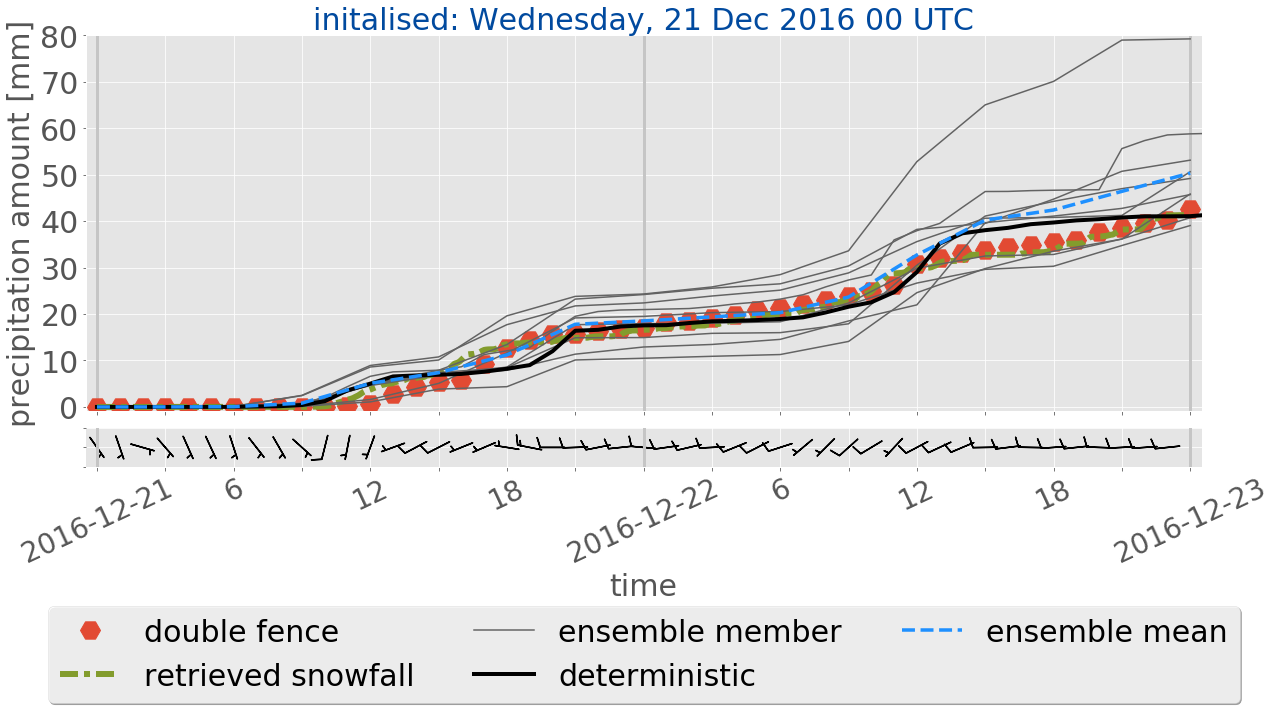
\includegraphics[trim={0.cm 5.2cm 0.cm 0cm},clip,width=\textwidth]{./fig_sfc_acc/acc_wind_20161221_00}
		\caption{}\label{fig:sfc_acc21}
	\end{subfigure}
	% 22/12
	\begin{subfigure}[t]{0.49\textwidth}		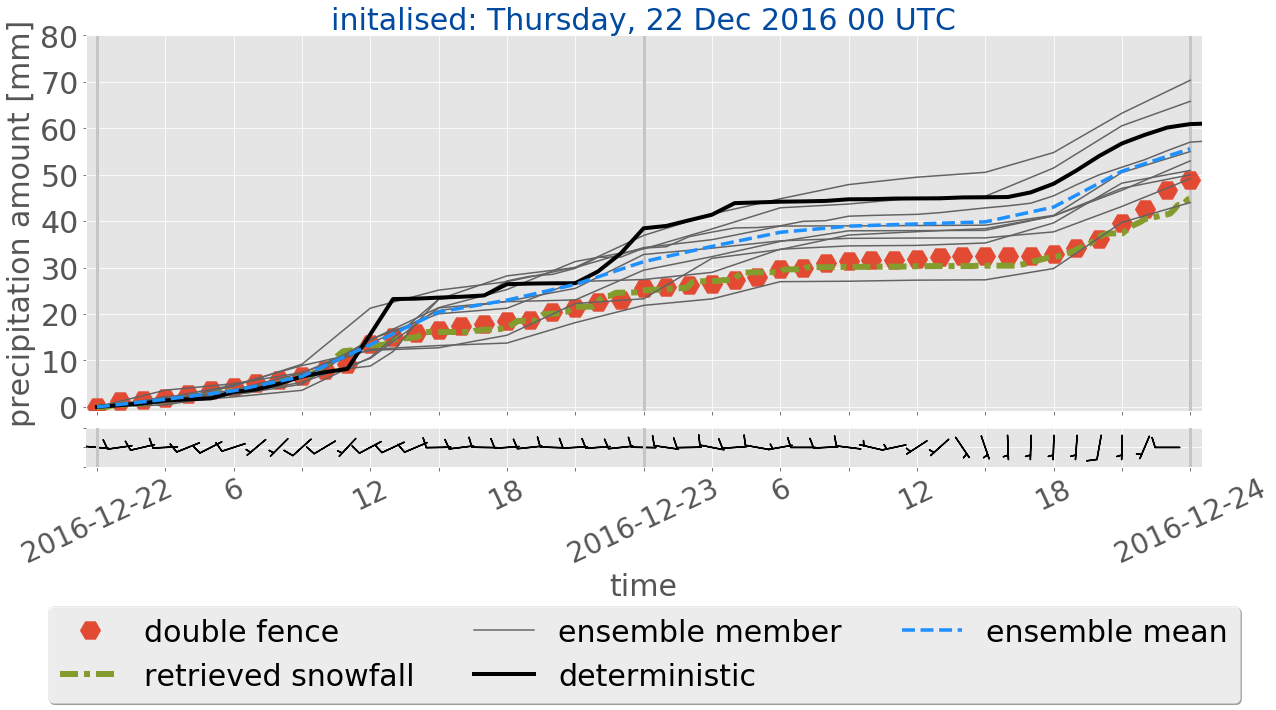
\includegraphics[trim={0.cm 5.2cm 0.cm 0cm},clip,width=\textwidth]{./fig_sfc_acc/acc_wind_20161222_00}
		\caption{}\label{fig:sfc_acc22}
	\end{subfigure}
	%	\end{figure}
	%   \begin{figure}\ContinuedFloat
	% 23/12
	\begin{subfigure}[t]{0.49\textwidth}	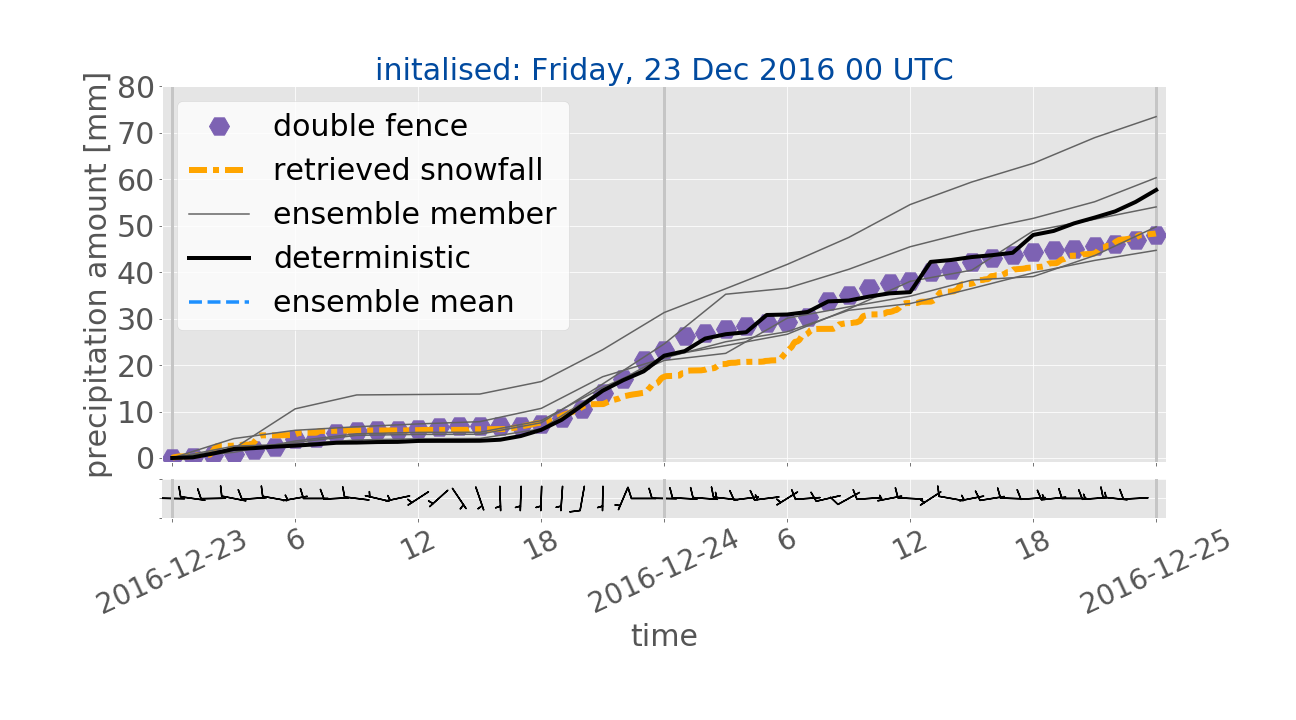
\includegraphics[trim={0.cm 5.2cm 0.cm 0cm},clip,width=\textwidth]{./fig_sfc_acc/acc_wind_20161223_00}
		\caption{}\label{fig:sfc_acc23}
	\end{subfigure}
	% 24/12
	\begin{subfigure}[t]{0.49\textwidth}			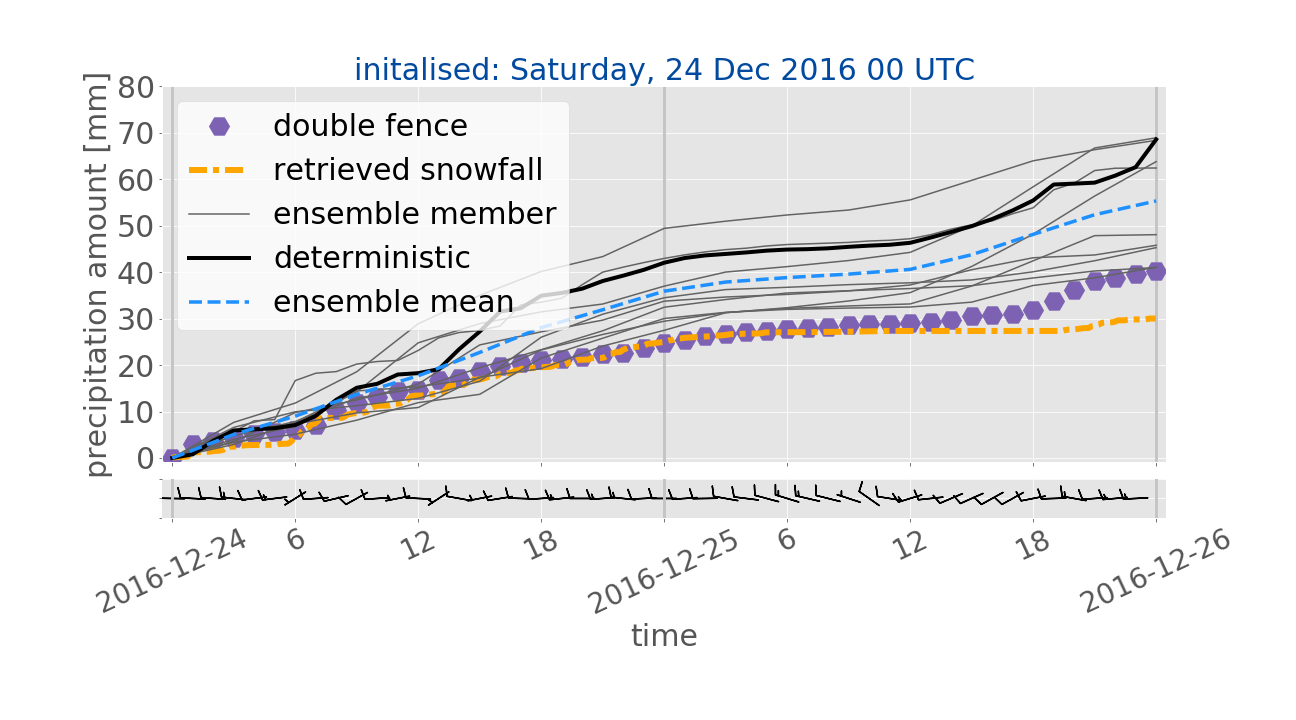
\includegraphics[trim={0.cm 5.2cm 0.cm 0cm},clip,width=\textwidth]{./fig_sfc_acc/acc_wind_20161224_00}
		\caption{}\label{fig:sfc_acc24}
	\end{subfigure}
	% 25/12
	\begin{subfigure}[t]{0.49\textwidth}
		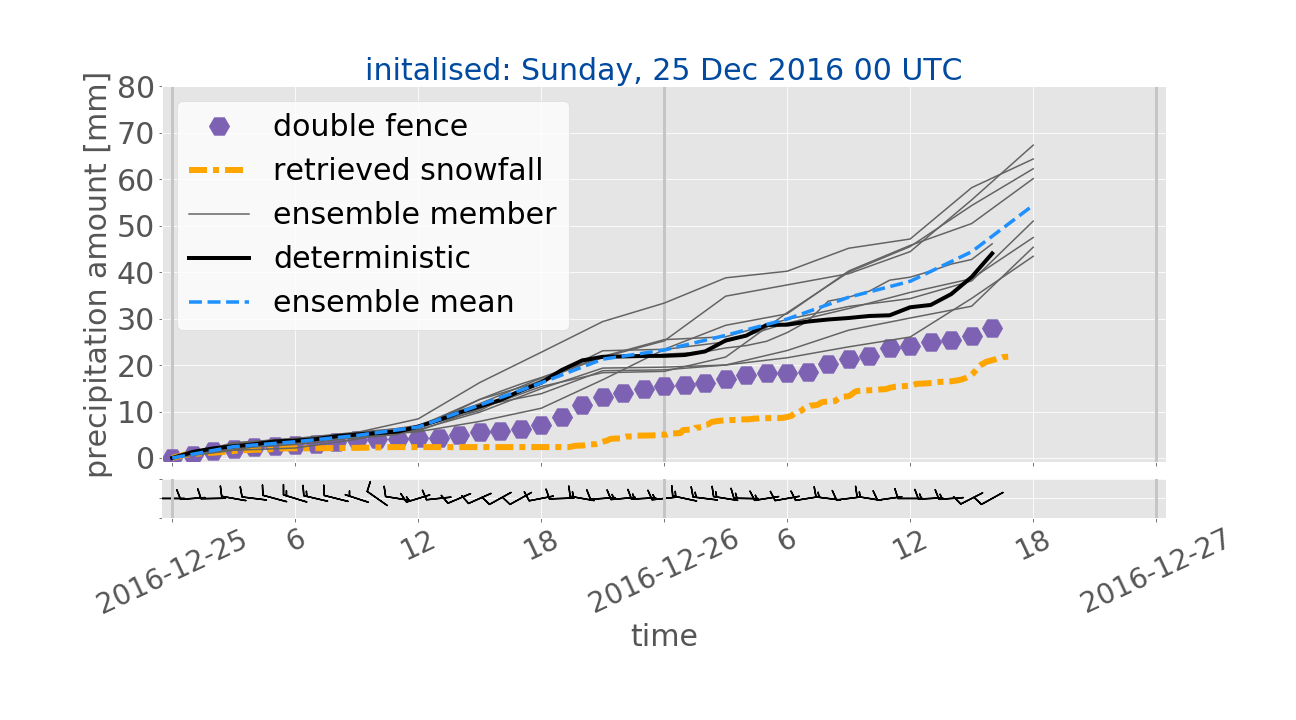
\includegraphics[trim={0.cm 3.6cm 0.cm 0cm},clip,width=\textwidth]{./fig_sfc_acc/acc_wind_20161225_00}
		\caption{}\label{fig:sfc_acc25}
	\end{subfigure}
	% 26/12
	\begin{subfigure}[t]{0.49\textwidth}	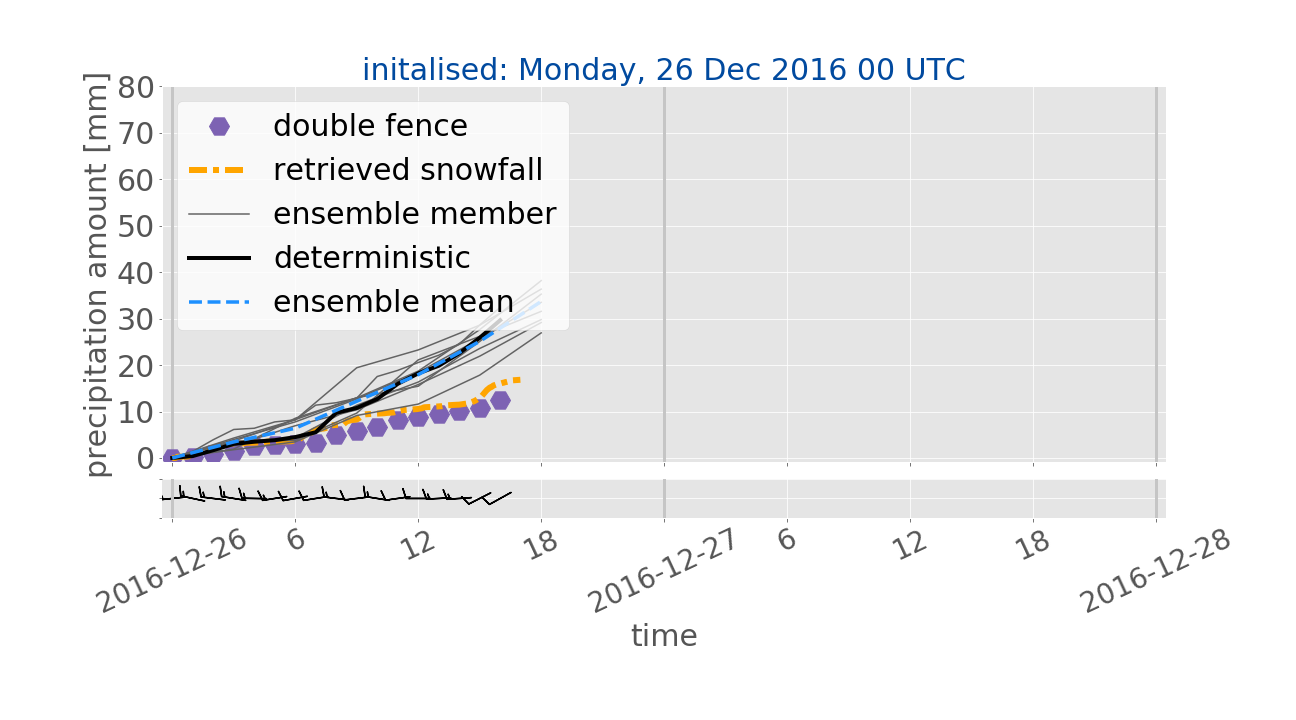
\includegraphics[trim={0.cm 3.6cm 0.cm 0cm},clip,width=\textwidth]{./fig_sfc_acc/acc_wind_20161226_00}
		\caption{}\label{fig:sfc_acc26}
	\end{subfigure}
	
	% label
	\begin{subfigure}[t]{\textwidth}
		\centering
		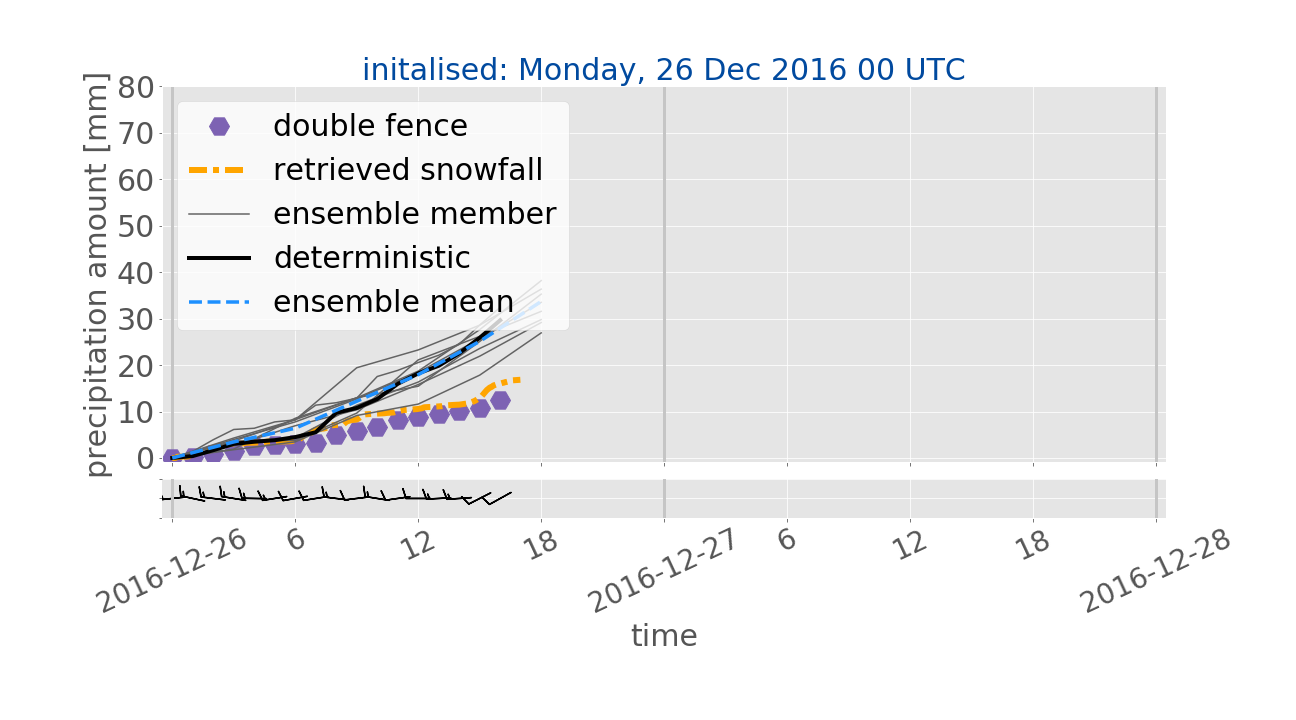
\includegraphics[trim={1.2cm 0cm 1.1cm 21.4cm},clip,width=0.8\textwidth]{./fig_sfc_acc/acc_wind_20161226_00}
	\end{subfigure}
	\caption{\SI{48}{\hour} surface snowfall accumulation for \SIrange{21}{26}{\dec} (\protect\subref{fig:sfc_acc21}  \protect\subref{fig:sfc_acc26}). Representing the values from the double fence in red, hexagons; optimal estimation retrieval output at snow layer height \SI{400}{\metre} in dash-dotted green; and ensemble member deterministic forecast, initialised at \SI{00}{\UTC} in black and its nine perturbed ensemble members in grey. The ensemble mean of all ten members is shown in dashed blue. Underneath are the associated last hour \SI{10}{\minute} average wind from the weather mast at \SI{10}{\metre} height. }\label{fig:sfc_acc}
\end{figure}
%%%%%%%%%%%%%%%%%%%%%%%%%%%%%%%%%%%%%%%%%%%%%%%%%%%%%%%%%%%%%%%%%%%%%%%%%%
One approach of this study is to see if observed surface accumulation was correctly predicted by the regional weather model MEPS. Precipitation amount at the surface are shown in \Cref{fig:sfc_acc}. The figures are representing the observed and forecasted surface precipitation accumulation in \SI{}{\mm} over \SI{48}{\hour}. Accumulation, measured by the double fence are presented as red hexagons. Minutely retrieved surface snowfall amount in dash-dotted green. The ten \SI{48}{\hour} forecast ensemble members are lines in black and grey, the deterministic and its perturbed ensemble members, respectively. The blue dashed line shows the ensemble mean of all ten members. Since the deterministic and the first ensemble member are having values every hour and the other perturbed members only every three hours, shows the ensemble mean the precipitation amount at \SI{0}{\hour}, \SI{3}{\hour}, $\ldots$, \SI{21}{\hour}, \SI{24}{\hour}, $\ldots$, \SI{48}{\hour} forecast time. When too few ensemble members were present, like on \SI{23}{\dec}, no ensemble mean is calculated (\Cref{fig:sfc_acc23}). 
Underneath is the associated \SI{10}{\minute} average wind of the last hour from the \SI{10}{\metre} weather mast at Haukeliseter, to see if surface accumulation observations may be influenced by wind. 
\\
\Cref{fig:sfc_acc21,fig:sfc_acc22,fig:sfc_acc23} show in general a better agreement between observations and forecast for \SI{48}{\hour} forecasts initialised on \SIrange{21}{23}{\dec} at \SI{0}{\UTC}. The spread of the ensemble members around the control run fit better to the observations as well than initialisations on \SIrange{24}{26}{\dec}. 
During these days intensifies the low-pressure system and gets closer advected to the Norwegian coast and influencing the local weather in Norway (\Cref{ch:weather_ana}). \Cref{fig:sfc_acc24,fig:sfc_acc25,fig:sfc_acc26} indicates a larger estimated surface precipitation amount for all ten ensemble members than observed at the measurement site between \SIrange{24}{26}{\dec}. 
\\ 
\\
The correlation between double fence observation and ensemble forecast is presented in \Cref{fig:scat:pres2123} and \subref{fig:scat:pres2426}. Showing a better agreement between \SIrange{21}{23}{\dec} than initialisation on \SIrange{24}{26}{\dec}. On \SIrange{21}{23}{\dec} is the slope of the regression relatively close to unity, indicating a good agreement between the ensemble forecast and the observations by the double fence.
The largest disagreement between surface observations and forecasts is seen on \SI{25}{\dec} with a positive bias up to \SI{17}{\mm} (\Cref{fig:bias:precip}). The mean absolute error is not larger than \SI{13}{\mm} for the first three days and increases with intensification of the storm up to \SI{19}{\mm} on \SI{24}{\dec}.
\\
Initialisations on \SI{24}{\dec} indicate an overestimation of the deterministic surface snowfall prediction already after \SI{13}{\hour} forecast time. The deterministic forecast in solid black is much higher and increases faster than the observations. In \Cref{fig:sfc_acc24} at \SI{16}{\UTC} a higher value of approximately \SI{15}{\mm} can be seen when compared to the surface measurements. This difference remains almost constantly over the forecast time. Furthermore, all ensemble members seem to overestimate the surface accumulation after \SI{24}{\hour} prediction time. 
\\
Since the MEPS performance was better on the previous days one might assume that the double fence measurement is influenced by surface winds. It shows in \Cref{fig:sfc_acc24} that the \SI{10}{\minute} average wind at \SI{13}{\UTC} increases from \SI{5}{\mPs} to \SI{10}{\mPs} (see also \Cref{fig:res:sfc_ws24}). \citet{wolff_wmo_2018} states that the double fence gauge is influenced by wind, but accumulation measurement errors occur rather at higher wind speeds larger than \SI{20}{\mPs}. It is therefore assumed that the measurements from the double fence are correct and MEPS had rather a forecasting issue.
\\
While the cyclone gets more advected to Norway increases the forecast inaccuracy of the surface precipitation. 
On \SI{25}{\dec} the miscalculation of the precipitation amount is associated with the warm sector passage at Haukeliseter (\Cref{sec:res:large_scale_sfc}). Afterwards follows the model the same path as the double fence observations, but higher. The \SI{25}{\dec} indicates a good spread between the ensemble members and the deterministic forecast, while on \SI{24}{\dec} the ensemble members were not spread symmetrically around the deterministic forecast. 
\\
An overestimation of the surface accumulation is also observed on \SI{26}{\dec}. While the large-scale analysis indicates the passage of an occlusion after \SI{15}{\UTC} (\Cref{fig:DT26}, \ref{fig:GP26}) seems the overestimation to occur after \SI{12}{\hour} forecast time in \Cref{fig:sfc_acc26}. Again, all ensemble members seem to follow the course of the double fence accumulation, but larger. 
\\
Whereas the spread between the ensemble members is large in the beginning of \SI{24}{\dec} is the variability between the members narrow for \SIlist{25;26}{\dec}. The variability between the ensemble member can be compared with a box-whisker plot. A box-whisker-plot shows the time evolution of the distribution of the precipitation amount made of ten ensemble members up to \SI{48}{\hour}. Since some ensemble member do not have forecast values every hour provides the box-whisker-plot in \Cref{fig:boxplot} information every \SI{3}{\hour}. The red line shows the ensemble mean of all ten members and shows if the distribution is skewed. The short light green horizontal line is showing the median, wide vertical box represents the 25th and 75th percentiles, and minimum and maximum values are indicated by the vertical lines, whiskers.
\\
%%% image surface accumulation %%%%%%%%%%%%%%%%%%%%%%%%%%%%%%%%%%%%%
\begin{figure}[h!]
	\centering
	\begin{subfigure}[b]{\textwidth}
		\centering
		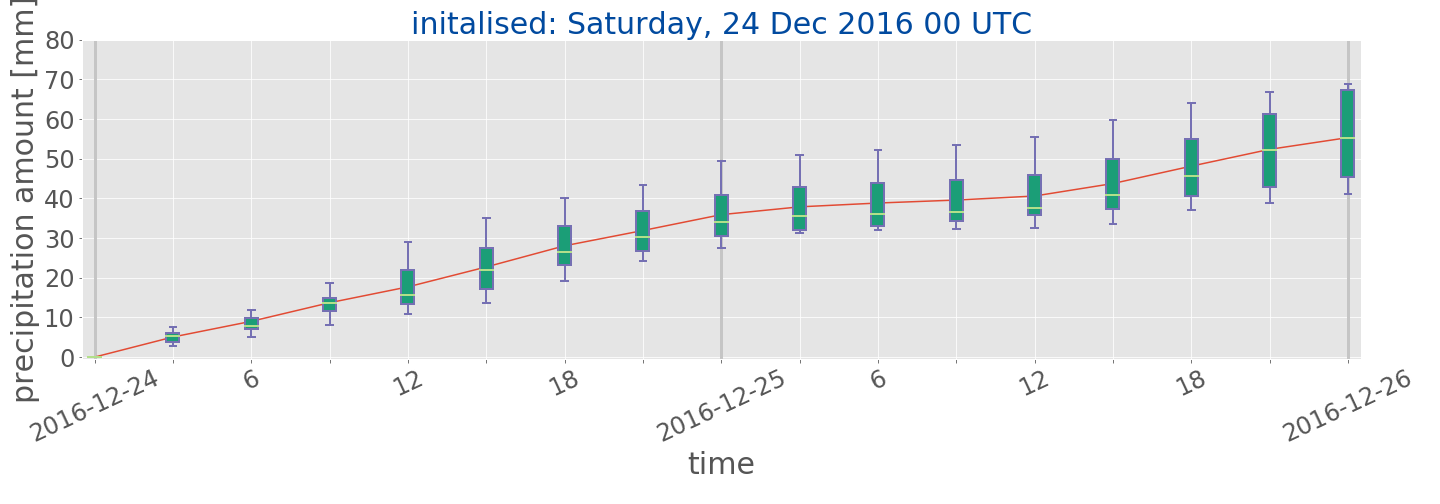
\includegraphics[trim ={0cm 2.2cm 0cm 0cm},clip,width=\textwidth]{./fig_boxplot_sfc/20161224_0}
		\caption{}\label{fig:boxplot:24}
	\end{subfigure}
	%
	\begin{subfigure}[b]{\textwidth}
		\centering
		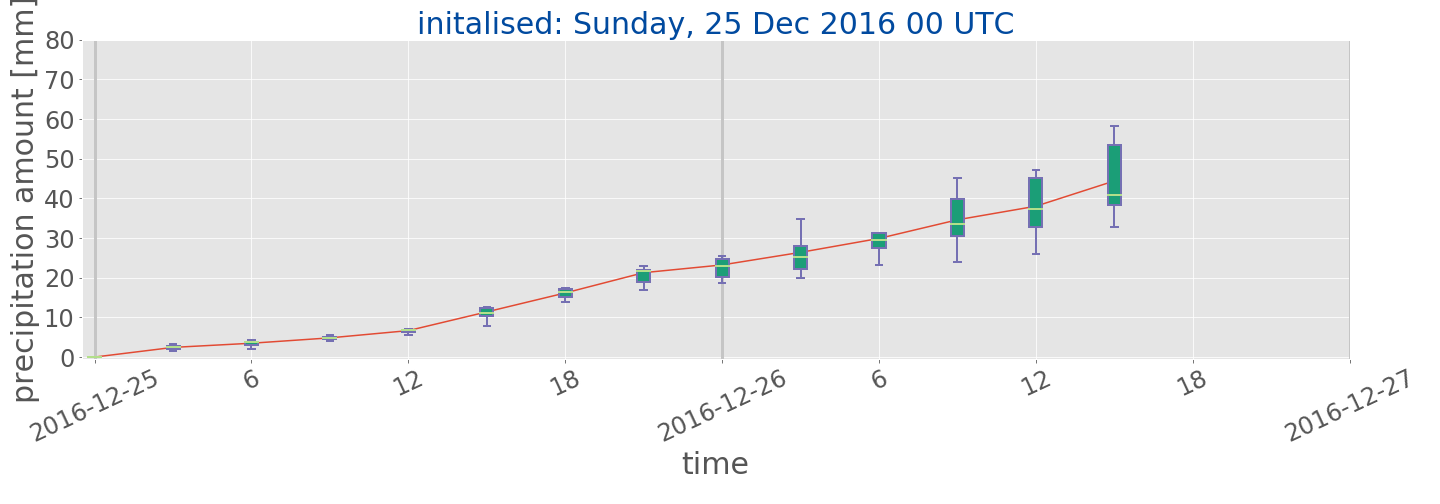
\includegraphics[trim ={0cm 2.2cm 0cm 0cm},clip,width=\textwidth]{./fig_boxplot_sfc/20161225_0}
		\caption{}\label{fig:boxplot:25}
	\end{subfigure}
	%
	\begin{subfigure}[b]{\textwidth}
		\centering
		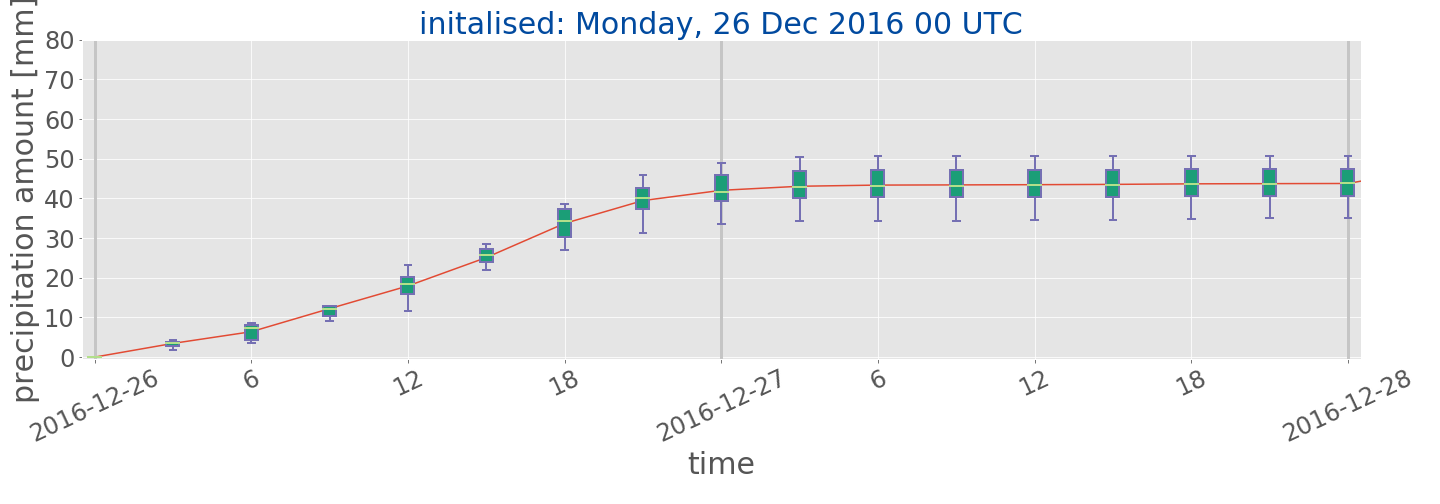
\includegraphics[trim ={0cm 1.cm 0cm 0cm},clip,width=\textwidth]{./fig_boxplot_sfc/20161226_0}
		\caption{}\label{fig:boxplot:26}
	\end{subfigure}
	\caption{Box-whisker-plot of the ten ensemble members of MEPS. Red line indicating the ensemble mean, lower and upper whisker the 25th and 75th percentile, respectively. Light green shows the median of all members and the box represents the middle \SI{50}{\percent} of scores of the precipitation.}\label{fig:boxplot}
\end{figure}
%%%%%%%%%%%%%%%%%%%%%%%%%%%%%%%%%%%%%%%%%%%%%%%%%%%%%%%%%%%%%%%%%%%%%%%%%%
\\
The box-whisker-plot in \Cref{fig:boxplot} shows the distribution of the ten ensemble members for the respective days. All three days with overestimation seem to be different in their variability. As expected increases the forecast uncertainty with longer forecast time for precipitation amount.  
\\
\Cref{fig:boxplot:25} shows for \SI{25}{\dec} the least variability between the ten ensemble members of up to almost \SI{24}{\hour}. The \SI{25}{\dec} is also the forecast with the smallest positive bias of these three days. As \Cref{fig:scat:precip2426} suggests is the overestimation not as high as for \SIlist{24;25}{\dec}. On \SIlist{24;26}{\dec} is the mean error for the surface accumulation largest with values up to \SI{19}{\mm}. 
\\
Larger variability is already present after \SI{3}{\hour} prediction time in \Cref{fig:boxplot:24} on \SI{24}{\dec}. The spread between the ensemble members (shown by the minimum and maximum whiskers) seems to be wide indicating a larger uncertainty about the amount of surface accumulation. The ensemble mean (red line) is always higher than the median and already after \SI{12}{\hour} forecast time is the median closer to the lower 25th percentile. Also, all upper whiskers in \Cref{fig:boxplot:24} are taller than the lower ones, which would follow that the ensemble members vary amongst the most positive quartile and that it is very similar for the least positive quartile group. Since the deterministic forecast, black line in \Cref{fig:sfc_acc24}, is in the upper percentile compared to its perturbed members it follows that for this forecast the deterministic forecast was not the best guess for the surface accumulation and by using the 'wrong' initial state it can have led to larger miscalculations. 
\\
I believe that the uncertainty appearing already after \SI{3}{\hour} could be associated with a too long spin-up time of MEPS. MEPS usually has a spin-up time of about three hours, on \SI{24}{\dec} this might have been longer as a result of poorer initial conditions \textcolor{red}{Need a reference here, not stated in \citet{muller_arome-metcoop:_2017}}. The regional model MEPS receives initial and boundary conditions from ECMWF before it can produce forecasts \citep{muller_arome-metcoop:_2017}. Since initial conditions such as observations have uncertainties as well as the model has mistrust, and  the own climatology needs to be approached, a model has to stabilize before the simulations can be trusted. The spin-up time varies depending on the quality of the initial and boundary conditions. Apparently, it seems, that the initial and boundary conditions for MEPS were not perfect for initialisations on \SI{24}{\dec} at \SI{0}{\UTC}. The deterministic and perturbed members seem not to have stabilised yet and show larger variability in \Cref{fig:boxplot24} from early on.
\\
The uncertainty might have also been related to the fact, that the large-scale situation got more complex. The precipitation amount associated with the passage of an occluded front on \SI{23}{\dec} was higher than on the previous days (\Cref{fig:res:sfc_precip23} and \Cref{fig:TPU}). On previous days was the hourly precipitation around \SI{0}{\UTC} less intense than on \SI{23}{\dec}. This led to a higher accumulation amount over shorter time and could have followed a larger variability in the forecast model. Another possibility is perhaps that MEPS might have accounted for additional precipitation around \SI{12}{\UTC} on \SI{24}{\dec} and this showed a stronger increase in accretion in \Cref{fig:sfc_acc24} at \SI{13}{\UTC}. I believe it could be associated to a local resolution effect of MEPS. \Cref{fig:meps:site} shows the MEPS resolution and its \SI{2.5}{\km} grid cells around the Haukeliseter site. The complex terrain represented in the model could have followed a local misplacement of a precipitation cell by a few kilometres and followed an estimation of more accumulation at the site after noon.
\\
\\
\Cref{fig:boxplot:25} and \subref{fig:boxplot:26} show a smaller ensemble member variability on \SIlist{25;26}{\dec} than on \SI{24}{\dec}. The box-whiskers are narrower for the first \SI{30}{\hour} in \Cref{fig:boxplot:25}, but slightly larger after \SI{6}{\hour} forecast time for initialisations on \SI{26}{\dec}. \Cref{sec:res:large_scale_sfc} presented a good agreement between observations and forecast of large scale features in terms of pressure, temperature and wind direction. While the occlusion on \SI{26}{\dec} was more intuitive (\Cref{fig:res:sfc_pres26,fig:res:sfc_temp26,fig:res:sfc_wd26,fig:res:sfc_ws26}) than the warm front passage on \SI{25}{\dec} (\Cref{fig:res:sfc_pres25}, \subref{fig:res:sfc_temp25}, \subref{fig:res:sfc_wd25}, \subref{fig:res:sfc_ws25}) shows the mean error for each variable to be best for \SI{25}{\dec} (\Cref{fig:MAE:pres},\subref{fig:MAE:temp},\subref{fig:MAE:wd}, \subref{fig:MAE:ws}, and \subref{fig:MAE:precip}).
\\
On \SI{25}{\dec}the overestimation started to occur around \SI{13}{\UTC} in \Cref{fig:sfc_acc25}, related to the delayed forecasted temperature increase in \Cref{fig:res:sfc_temp25}.  As \Cref{fig:boxplot25} shows, increases the variability in the forecast after \SI{15}{\hour} prediction time. In general, agree median and mean well for the entire period of a \SI{48}{\hour} forecast. After \SI{39}{\hour} prediction time is the mean much higher than the median and closer to the lower 25th percentile in \Cref{fig:boxplot25}. It seems, that all ten ensemble members agree well on the prediction and nevertheless overestimates MEPS the surface accumulation. I consider that MEPS misinterpreted the amount of precipitation related to the passage of the warm sector.  
\\
During \SI{26}{\dec} the core of the low-pressure system goes through between \SIlist{15;18}{\UTC} at Haukeliseter. The box-whiskers in \Cref{fig:boxplot:26} indicates a larger variability after \SI{6}{\hour} prediction while the precipitation amount forecast is miscalculated at \SI{12}{\UTC} and following the structure of the double fence observation. Variability of all ensemble members show to increase at \SI{6}{\hour} forecast time, but then decreases again in \Cref{fig:boxplot:26}.  
\\
Since the box-whisker-plot in \Cref{fig:boxplot:25} and \subref{fig:boxplot:26} show less variability in the beginning it is assumed that spin-up time issues are less likely. It could be related to an error in the initialisation state, even though it does not show in the variability in the beginning. An error associated with the spin-up time of MEPS is not totally excluded for these days. In \Cref{fig:sfc_acc25} and \subref{fig:sfc_acc26} agrees the ensemble mean well with the deterministic forecast, which is an indication of a symmetrical spread around the deterministic run. 
\\ 
The overestimation during \SIlist{24;26}{\dec} might be related to the high forecasted wind speeds, as well as to the complex development of the low-pressure system north-west of Norway on \SI{24}{\dec}.
\\
%%% table surface accumulation %%%%%%%%%%%%%%%%%%%%%%%%%%%%%%%%%%%%%
\begin{table}[h]
	\begin{center}
		\caption{Surface snowfall accumulation measured by the double fence gauge. Presenting \SI{12}{\hour} accumulation before noon and after noon, as well as the total \SI{24}{\hour} surface accretion. }\label{tab:sfc_acc}
		\begin{tabular}{c|c|c|c}
			\hline \hline
			\textbf{Day} & \multicolumn{3}{c}{\textbf{Accumulation}} \\ 
			& \multicolumn{3}{c}{[\SI{}{\mm}]} \\ \hline
			& \SI{12}{\hour} (\footnotesize{\num{0} to \SI{12}{\UTC}}) & \SI{12}{\hour} (\footnotesize{\num{12} to \SI{23}{\UTC}}) & \SI{24}{\hour} \\ \hline \hline
			\SI{21}{\dec} & \num{0.7} &  \num{16.4} & \num{17.1} \\ \hline
			\SI{22}{\dec} & \num{13.6} &  \num{12.0} & \num{25.6} \\ \hline
			\SI{23}{\dec} & \num{6.3} &  \num{17.0} & \num{23.3} \\ \hline
			\SI{24}{\dec} & \num{14.7} &  \num{10.1} & \num{24.8} \\ \hline
			\SI{25}{\dec} & \num{4.3} &  \num{11.1} & \num{15.4} \\ \hline
			\SI{26}{\dec} & \num{8.8} &  \num{16.3} & \num{25.1} \\ 
			\hline \hline
		\end{tabular}
	\end{center}
\end{table}
%%%%%%%%%%%%%%%%%%%%%%%%%%%%%%%%%%%%%%%%%%%%%%%%%%%%%%%%%%%%%%%%%%%%%%%%%%
\\
According to \citet{muller_arome-metcoop:_2017} are strong precipitation events better predicted with AROME-MetCoOp than with ECMWF (European Centre for Medium-Range Weather Forecasts). In \Cref{sec:dim:dec_obs} it was described, that during \SIrange{21}{27}{\dec} \SI{56.9}{\percent} of the total December 2016 accumulation were observed. \citet{muller_arome-metcoop:_2017} states also, that an overestimation appears, where the precipitation event (\SI{12}{\hour} accumulation) is less than \SI{10}{\mm} this seems not to be true for all days but could be possible for \SIlist{25;26}{\dec} (observed accumulation in \Cref{tab:sfc_acc}). In December 2014 was the \SI{12}{\hour} precipitation mean absolute error in AROME-MetCoOp with \SI{1.5}{\mm}. For the Christmas storm is the mean absolute error not larger than \SI{5}{\mm} for the first \SI{12}{\hour} accumulation on \SIlist{24;26}{\dec} (\Cref{fig:MAE:precip12}). Therefore, the assumption follows that on \SI{26}{\dec} the overestimation might be correlated to the <\SI{10}{\mm} problem described by \citet{muller_arome-metcoop:_2017}. The \SI{12}{\hour} accumulation is presented in \Cref{tab:sfc_acc} for Haukeliseter and shows that \SI{12}{\hour} accrection was less than \SI{10}{\mm} for \SIlist{25;26}{\dec}.
On \SI{25}{\dec} the mean absolute error was \SI{1.1}{\mm} for the first \SI{12}{\hour} accumulation and shows that this could be an influence but does not necessarily mean to be the case, since the overestimation started to occur after \SI{11}{\hour} prediction time. 
\\
\\
% keep as summary in the end
It will be interesting to re-run the ensemble prediction system again with all available observations to see, if this has an influence on the overestimation indicated in \Cref{fig:sfc_acc24,fig:sfc_acc25,fig:sfc_acc26}. ECMWF as boundary condition might not have reached its stabilised state itself when MEPS was initiated and could also have led to a misinterpretation of surface accumulation. A re-run with analysis data from ECMWF could possibly improve the original forecast \textcolor{red}{find reference for this}. 
Another approach could be to perturb the initial state (deterministic forecast) in other way, to see if different perturbations might lead to a better correlation between observation and forecast at the ground than presented in \Cref{fig:scat:precip2124}. Also, the deterministic forecast (best guess) might have been chosen incorrectly and followed a miscalculation of surface accumulation, since the misinterpreted best guess was perturbed.
It is very important to have correct measurements such as the double fence or MRR observations, to produce better initial condition for weather forecast models, so that initialisations can start at a realistic state.
\\
Also, more study cases should be considered to get a better estimate about the performance of MEPS during extreme winter events. The mean absolute error for \SI{12}{\hour} accumulation has shown a great variability, depending on the initialisation time and the intensification of the low-pressure system.  
%%%%%%%%%%%%%%%%%%%%%%%%%%%%%%%%%%%%%%%%%%%%%%%%%%%%%%%%%%%%%%%%%%%%%%%%%%




